% Options for packages loaded elsewhere
\PassOptionsToPackage{unicode}{hyperref}
\PassOptionsToPackage{hyphens}{url}
%
\documentclass[
]{book}
\usepackage{amsmath,amssymb}
\usepackage{iftex}
\ifPDFTeX
  \usepackage[T1]{fontenc}
  \usepackage[utf8]{inputenc}
  \usepackage{textcomp} % provide euro and other symbols
\else % if luatex or xetex
  \usepackage{unicode-math} % this also loads fontspec
  \defaultfontfeatures{Scale=MatchLowercase}
  \defaultfontfeatures[\rmfamily]{Ligatures=TeX,Scale=1}
\fi
\usepackage{lmodern}
\ifPDFTeX\else
  % xetex/luatex font selection
\fi
% Use upquote if available, for straight quotes in verbatim environments
\IfFileExists{upquote.sty}{\usepackage{upquote}}{}
\IfFileExists{microtype.sty}{% use microtype if available
  \usepackage[]{microtype}
  \UseMicrotypeSet[protrusion]{basicmath} % disable protrusion for tt fonts
}{}
\makeatletter
\@ifundefined{KOMAClassName}{% if non-KOMA class
  \IfFileExists{parskip.sty}{%
    \usepackage{parskip}
  }{% else
    \setlength{\parindent}{0pt}
    \setlength{\parskip}{6pt plus 2pt minus 1pt}}
}{% if KOMA class
  \KOMAoptions{parskip=half}}
\makeatother
\usepackage{xcolor}
\usepackage{color}
\usepackage{fancyvrb}
\newcommand{\VerbBar}{|}
\newcommand{\VERB}{\Verb[commandchars=\\\{\}]}
\DefineVerbatimEnvironment{Highlighting}{Verbatim}{commandchars=\\\{\}}
% Add ',fontsize=\small' for more characters per line
\usepackage{framed}
\definecolor{shadecolor}{RGB}{248,248,248}
\newenvironment{Shaded}{\begin{snugshade}}{\end{snugshade}}
\newcommand{\AlertTok}[1]{\textcolor[rgb]{0.94,0.16,0.16}{#1}}
\newcommand{\AnnotationTok}[1]{\textcolor[rgb]{0.56,0.35,0.01}{\textbf{\textit{#1}}}}
\newcommand{\AttributeTok}[1]{\textcolor[rgb]{0.13,0.29,0.53}{#1}}
\newcommand{\BaseNTok}[1]{\textcolor[rgb]{0.00,0.00,0.81}{#1}}
\newcommand{\BuiltInTok}[1]{#1}
\newcommand{\CharTok}[1]{\textcolor[rgb]{0.31,0.60,0.02}{#1}}
\newcommand{\CommentTok}[1]{\textcolor[rgb]{0.56,0.35,0.01}{\textit{#1}}}
\newcommand{\CommentVarTok}[1]{\textcolor[rgb]{0.56,0.35,0.01}{\textbf{\textit{#1}}}}
\newcommand{\ConstantTok}[1]{\textcolor[rgb]{0.56,0.35,0.01}{#1}}
\newcommand{\ControlFlowTok}[1]{\textcolor[rgb]{0.13,0.29,0.53}{\textbf{#1}}}
\newcommand{\DataTypeTok}[1]{\textcolor[rgb]{0.13,0.29,0.53}{#1}}
\newcommand{\DecValTok}[1]{\textcolor[rgb]{0.00,0.00,0.81}{#1}}
\newcommand{\DocumentationTok}[1]{\textcolor[rgb]{0.56,0.35,0.01}{\textbf{\textit{#1}}}}
\newcommand{\ErrorTok}[1]{\textcolor[rgb]{0.64,0.00,0.00}{\textbf{#1}}}
\newcommand{\ExtensionTok}[1]{#1}
\newcommand{\FloatTok}[1]{\textcolor[rgb]{0.00,0.00,0.81}{#1}}
\newcommand{\FunctionTok}[1]{\textcolor[rgb]{0.13,0.29,0.53}{\textbf{#1}}}
\newcommand{\ImportTok}[1]{#1}
\newcommand{\InformationTok}[1]{\textcolor[rgb]{0.56,0.35,0.01}{\textbf{\textit{#1}}}}
\newcommand{\KeywordTok}[1]{\textcolor[rgb]{0.13,0.29,0.53}{\textbf{#1}}}
\newcommand{\NormalTok}[1]{#1}
\newcommand{\OperatorTok}[1]{\textcolor[rgb]{0.81,0.36,0.00}{\textbf{#1}}}
\newcommand{\OtherTok}[1]{\textcolor[rgb]{0.56,0.35,0.01}{#1}}
\newcommand{\PreprocessorTok}[1]{\textcolor[rgb]{0.56,0.35,0.01}{\textit{#1}}}
\newcommand{\RegionMarkerTok}[1]{#1}
\newcommand{\SpecialCharTok}[1]{\textcolor[rgb]{0.81,0.36,0.00}{\textbf{#1}}}
\newcommand{\SpecialStringTok}[1]{\textcolor[rgb]{0.31,0.60,0.02}{#1}}
\newcommand{\StringTok}[1]{\textcolor[rgb]{0.31,0.60,0.02}{#1}}
\newcommand{\VariableTok}[1]{\textcolor[rgb]{0.00,0.00,0.00}{#1}}
\newcommand{\VerbatimStringTok}[1]{\textcolor[rgb]{0.31,0.60,0.02}{#1}}
\newcommand{\WarningTok}[1]{\textcolor[rgb]{0.56,0.35,0.01}{\textbf{\textit{#1}}}}
\usepackage{longtable,booktabs,array}
\usepackage{calc} % for calculating minipage widths
% Correct order of tables after \paragraph or \subparagraph
\usepackage{etoolbox}
\makeatletter
\patchcmd\longtable{\par}{\if@noskipsec\mbox{}\fi\par}{}{}
\makeatother
% Allow footnotes in longtable head/foot
\IfFileExists{footnotehyper.sty}{\usepackage{footnotehyper}}{\usepackage{footnote}}
\makesavenoteenv{longtable}
\usepackage{graphicx}
\makeatletter
\def\maxwidth{\ifdim\Gin@nat@width>\linewidth\linewidth\else\Gin@nat@width\fi}
\def\maxheight{\ifdim\Gin@nat@height>\textheight\textheight\else\Gin@nat@height\fi}
\makeatother
% Scale images if necessary, so that they will not overflow the page
% margins by default, and it is still possible to overwrite the defaults
% using explicit options in \includegraphics[width, height, ...]{}
\setkeys{Gin}{width=\maxwidth,height=\maxheight,keepaspectratio}
% Set default figure placement to htbp
\makeatletter
\def\fps@figure{htbp}
\makeatother
\setlength{\emergencystretch}{3em} % prevent overfull lines
\providecommand{\tightlist}{%
  \setlength{\itemsep}{0pt}\setlength{\parskip}{0pt}}
\setcounter{secnumdepth}{5}
\usepackage{booktabs}
\usepackage{titling}
\usepackage{tcolorbox}
\tcbuselibrary{listings, theorems}
\usepackage{enumitem}
\usepackage{setspace}\onehalfspacing
\usepackage{fancyhdr}
\usepackage{hyphenat}
\usepackage{eso-pic,graphicx}
\usepackage{transparent}
\usepackage{draftwatermark}
\usepackage{amsmath}
\usepackage{hyperref}
\pagestyle{fancy}
\usepackage{caption}
\usepackage{theorem}
\usepackage[bahasai]{babel}
\ifLuaTeX
  \usepackage{selnolig}  % disable illegal ligatures
\fi
\usepackage[]{natbib}
\bibliographystyle{plainnat}
\IfFileExists{bookmark.sty}{\usepackage{bookmark}}{\usepackage{hyperref}}
\IfFileExists{xurl.sty}{\usepackage{xurl}}{} % add URL line breaks if available
\urlstyle{same}
\hypersetup{
  pdftitle={Modul Analisis Deret Waktu - AK2281},
  pdfauthor={Leonardo V Kosasih, S.Aktr, ASAI},
  hidelinks,
  pdfcreator={LaTeX via pandoc}}

\title{Modul Analisis Deret Waktu - AK2281}
\author{Leonardo V Kosasih, S.Aktr, ASAI}
\date{}

\begin{document}
\maketitle

{
\setcounter{tocdepth}{1}
\tableofcontents
}
\newtcbtheorem[auto counter]{jp}{Jurnal Praktikum}{fonttitle=\bfseries\upshape, fontupper=\slshape, arc=0mm, colback=blue!5!white,colframe=blue!75!black}{jurnal}

\hypertarget{selamat-datang}{%
\chapter*{Selamat Datang !}\label{selamat-datang}}
\addcontentsline{toc}{chapter}{Selamat Datang !}

\hypertarget{kata-pengantar}{%
\section*{Kata Pengantar}\label{kata-pengantar}}
\addcontentsline{toc}{section}{Kata Pengantar}

Puji dan syukur saya ucapkan kepada Lorem Ipsum

\hypertarget{kontak-penulis}{%
\section*{Kontak Penulis}\label{kontak-penulis}}
\addcontentsline{toc}{section}{Kontak Penulis}

\begin{itemize}
\tightlist
\item
  Github: \href{https://github.com/leonv1602}{leonv1602}\\
\item
  LinkedIn: \href{https://www.linkedin.com/in/leonardo-valentino-kosasih-4203a1182/}{Leonardo V Kosasih}
\end{itemize}

\hypertarget{penyusun-modul}{%
\section*{Penyusun Modul}\label{penyusun-modul}}
\addcontentsline{toc}{section}{Penyusun Modul}

Koordinator Praktikum : Leonardo V. Kosasih, S.Aktr., ASAI\\
Tim Penyusun Modul Praktikum :

\begin{longtable}[]{@{}
  >{\raggedright\arraybackslash}p{(\columnwidth - 2\tabcolsep) * \real{0.5000}}
  >{\raggedright\arraybackslash}p{(\columnwidth - 2\tabcolsep) * \real{0.5000}}@{}}
\toprule\noalign{}
\endhead
\bottomrule\noalign{}
\endlastfoot
Ang Ditra Alif Pradana-10120046 & Matthew Alfarazh - 10820021 \\
Feby Yolanda - 10819028 & Pamella Cathryn - 10820033 \\
Ferdinan Gratius Budisatya - 10819041 & Jeremy - 10820034 \\
Jevan Christopher Aryento - 10820010 & Aloysius Vincent - 10820038 \\
Shelly Delfiani - 10820014 & Kevin Christ Aditya - 10820039 \\
Binsar Gunadi Simbolon - 10820017 & Shafina Aulia Kusuma Putri - 10820049 \\
\end{longtable}

\hypertarget{daftar-notasi-dan-simbol-yang-digunakan}{%
\section*{Daftar Notasi dan Simbol yang Digunakan}\label{daftar-notasi-dan-simbol-yang-digunakan}}
\addcontentsline{toc}{section}{Daftar Notasi dan Simbol yang Digunakan}

\begin{itemize}
\tightlist
\item
  \(\varepsilon_t\)(baca : epsilon) : galat ke-\(t\);\\
\item
  \(\gamma_k\) (baca : gamma) : kovariansi ke-\(k\);\\
\item
  \(\rho_k\) (baca : rho) : korelasi ke-\(k\);\\
\item
  \(\phi_{ij}\) (baca : phi) : korelasi parsial antara \(i\) dan \(j\);\\
\item
  \(X \sim \text{N}(0,\sigma^2)\) : Peubah acak \(X\) berdistribusi Normal dengan rataan 0 dan variansi \(\sigma^2\);\\
\item
  ACF : \emph{Auto Correlation Function} atau Fungsi Auto korelasi;\\
\item
  PACF : \emph{Partial Auto Correlation Function} atau Fungsi Auto Korelasi Parsial;\\
\item
  \(\mathbb{N}\) : Himpunan bilangan asli \(\{1,2,3,\dots\}\);\\
\item
  \(\mathbb{N}_0\) : Himpunan bilangan asli dan 0 \(\{0,1,2,3,\dots\}\);\\
\item
  \(\sigma^2_\varepsilon\) (baca : sigma) : variansi dari \(\varepsilon\);\\
\item
  \(\bar{x}\) : rataan dari \(x\);\\
\item
  \(\theta\) (baca : theta);\\
\item
  \(\chi^2\) (baca : \emph{chi-squared});\\
\item
  \(\mathbf{A}\) : matriks \(A\) ukuran \(k\times k\);\\
\item
  \(\in\) : elemen dari suatu himpunan.\\
\item
  \(\forall\) : untuk setiap
\end{itemize}

\hypertarget{konsep-dasar-deret-waktu}{%
\chapter{Konsep Dasar Deret Waktu}\label{konsep-dasar-deret-waktu}}

\hypertarget{tujuan}{%
\section{Tujuan}\label{tujuan}}

\begin{enumerate}
\def\labelenumi{\arabic{enumi}.}
\tightlist
\item
  Memahami pola data deret waktu,\\
\item
  Mengidentifikasi deret waktu stasioner,\\
\item
  Menghitung rataan, kovariansi dan korelasi pada deret waktu\\
\item
  Mengenal model \emph{random walk}.\\
\item
  Mengidentifikasi perilaku ACF dan PACF.
\end{enumerate}

\hypertarget{stasioneritas}{%
\section{Stasioneritas}\label{stasioneritas}}

Asumsi yang harus dipenuhi pada pemodelan deret waktu adalah \textbf{stasioneritas}. Ide dasar dari kestasioneran adalah perilaku data tidak berubah sepanjang waktu. Ada 2 jenis stasioneritas yaitu \textbf{stasioneritas kuat} dan \textbf{stasioneritas lemah}. Misal proses \(\{Y_t\}\) dengan rataan \(\mu_t\). \(\{Y_t\}\) dikatakan \textbf{stasioner kuat} jika distribusi gabungan dari \(Y_{t_1},Y_{t_2},\dots,Y_{t_n}\) sama dengan distribusi gabungan \(Y_{t_1-k},Y_{t_2-k},\dots,Y_{t_n-k}\) untuk semua waktu \(t_1,t_2,\dots,t_n\) dan lag waktu \(k>0\).\\
Contoh : proses white noise \(\{\varepsilon_t\}\) dengan \(\varepsilon_t \sim \text{N}(0, \sigma^2)\) saling bebas dan indentik.\\
Sedangkan proses stokastik \(\{Y_t \}\) dikatakan \textbf{stasioner lemah} jika:\\
1. Rataan konstan sepanjang waktu atau \(E[Y_t] = \mu \quad \forall t \in \mathbb{N}_0\); dan\\
2. Kovariansi untuk semua waktu \(t\) dan lag \(k\) konstan atau \(\text{Cov}(Y_t,Y_{t-k}) = \gamma_{t,t-k} = \gamma_{0,k} = \gamma_k\).

Pada modul ini hanya dibahas tentang sifat kestasioneran lemah.

Beberapa contoh pola data dalam deret waktu, diantaranya pola tren, musiman, dan pola stasioner.\\
1. Pola tren: Terjadi jika terdapat kenaikan atau penurunan sekuler jangka panjang dalam data;\\
2. Pola musiman: Terjadi jika suatu deret dipengaruhi oleh faktor musiman (misalnya kuartal tahun, bulanan, atau hari-hari pada minggu tertentu); dan\\
3. Pola stasioner: Terjadi jika data berfluktuasi di sekitar rata-rata yang konstan.

\begin{Shaded}
\begin{Highlighting}[]
\CommentTok{\# Package yang digunakan }
\FunctionTok{library}\NormalTok{(zoo)}
\FunctionTok{library}\NormalTok{(forecast)}
\FunctionTok{library}\NormalTok{(tseries)}

\CommentTok{\# Seed agar simulasi tetap sama}
\FunctionTok{set.seed}\NormalTok{(}\DecValTok{1602}\NormalTok{)}

\CommentTok{\# Contoh data White Noise}
\NormalTok{wn }\OtherTok{\textless{}{-}} \FunctionTok{arima.sim}\NormalTok{(}\AttributeTok{model =}\FunctionTok{list}\NormalTok{(}\AttributeTok{order =} \FunctionTok{c}\NormalTok{(}\DecValTok{0}\NormalTok{,}\DecValTok{0}\NormalTok{,}\DecValTok{0}\NormalTok{)),}\AttributeTok{n =}\DecValTok{300}\NormalTok{)}
\FunctionTok{plot}\NormalTok{(wn, }\AttributeTok{main =} \StringTok{\textquotesingle{}Data 1, Stasioner\textquotesingle{}}\NormalTok{)}
\FunctionTok{abline}\NormalTok{(}\AttributeTok{h=}\FunctionTok{mean}\NormalTok{(wn),}\AttributeTok{col=}\StringTok{\textquotesingle{}red\textquotesingle{}}\NormalTok{,}\AttributeTok{lwd=}\DecValTok{2}\NormalTok{,}\AttributeTok{lty =} \DecValTok{2}\NormalTok{)}
\end{Highlighting}
\end{Shaded}

\begin{center}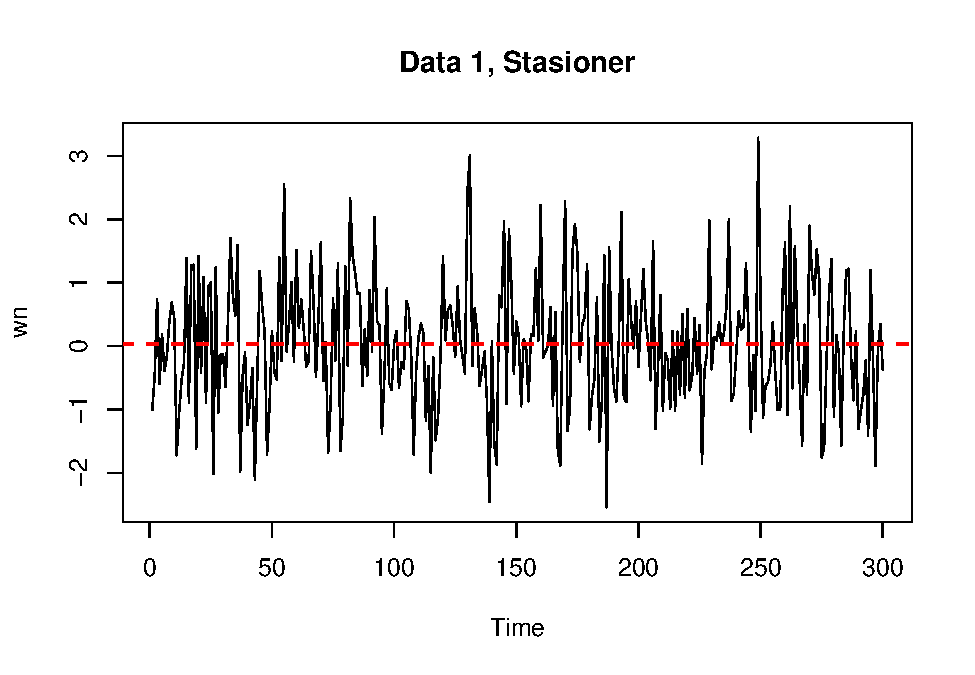
\includegraphics{_main_files/figure-latex/Contoh Plot yang Stasioner dan Tidak Stasioner-1} \end{center}

\begin{longtable}[]{@{}l@{}}
\toprule\noalign{}
Jurnal Praktikum 1 \\
\midrule\noalign{}
\endhead
\bottomrule\noalign{}
\endlastfoot
1. Berikan interpretasi anda terhadap gambar tersebut ! \\
2. Apakah data tersebar pada rataan data ? \\
3. Apakah terdapat pola tren data ? \\
\end{longtable}

\begin{Shaded}
\begin{Highlighting}[]
\CommentTok{\# Seed agar simulasi tetap sama}
\FunctionTok{set.seed}\NormalTok{(}\DecValTok{1602}\NormalTok{)}

\CommentTok{\# Data Harga Emas}
\FunctionTok{data}\NormalTok{(gold)}
\NormalTok{sum }\OtherTok{\textless{}{-}} \FunctionTok{ts}\NormalTok{(gold[}\DecValTok{1}\SpecialCharTok{:}\DecValTok{300}\NormalTok{])}
\NormalTok{sum }\OtherTok{\textless{}{-}} \FunctionTok{na.fill}\NormalTok{(sum,}\FunctionTok{median}\NormalTok{(sum,}\AttributeTok{na.rm=}\ConstantTok{TRUE}\NormalTok{))}
\NormalTok{mean\_sum }\OtherTok{\textless{}{-}} \FunctionTok{mean}\NormalTok{(sum,}\AttributeTok{na.rm=}\ConstantTok{TRUE}\NormalTok{)}
\FunctionTok{plot}\NormalTok{(sum, }\AttributeTok{main =} \StringTok{\textquotesingle{}Data Harga Emas, Tidak Stasioner\textquotesingle{}}\NormalTok{)}
\FunctionTok{abline}\NormalTok{(}\AttributeTok{h=}\NormalTok{mean\_sum,}\AttributeTok{col=}\StringTok{\textquotesingle{}red\textquotesingle{}}\NormalTok{,}\AttributeTok{lwd=}\DecValTok{2}\NormalTok{,}\AttributeTok{lty =} \DecValTok{2}\NormalTok{)}
\end{Highlighting}
\end{Shaded}

\begin{center}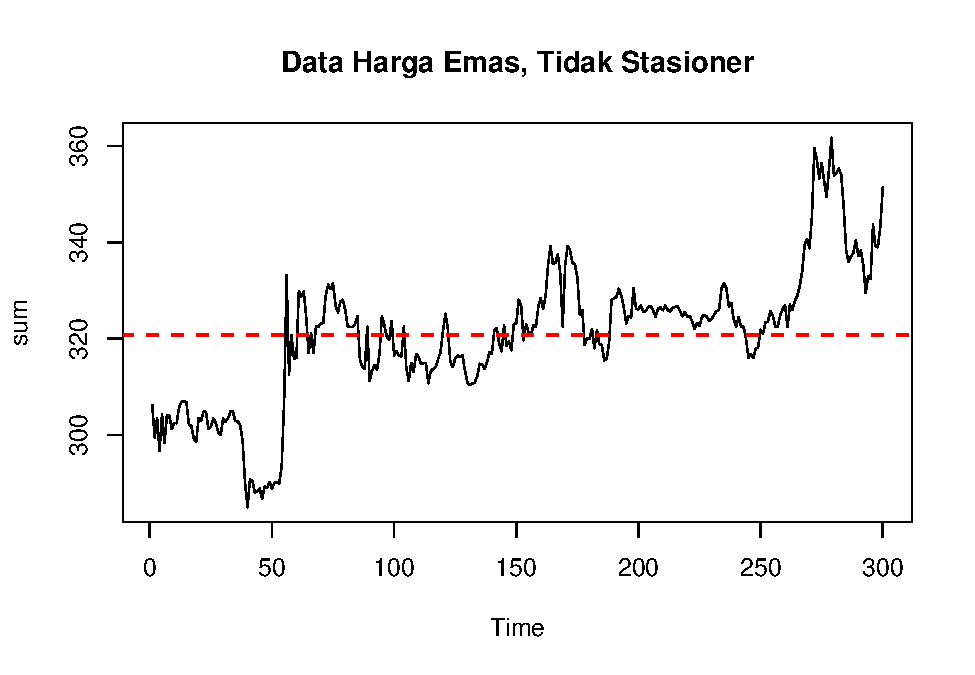
\includegraphics{_main_files/figure-latex/Contoh Plot yang Stasioner an Tidak Stasioner-1} \end{center}

\begin{longtable}[]{@{}l@{}}
\toprule\noalign{}
Jurnal Praktikum 2 \\
\midrule\noalign{}
\endhead
\bottomrule\noalign{}
\endlastfoot
1. Berikan interpretasi anda terhadap gambar tersebut ! \\
2. Apakah data tersebar pada rataan data ? \\
3. Apakah terdapat pola tren data ? \\
\end{longtable}

\begin{Shaded}
\begin{Highlighting}[]
\CommentTok{\# Seed agar simulasi tetap sama}
\FunctionTok{set.seed}\NormalTok{(}\DecValTok{1602}\NormalTok{)}

\CommentTok{\# Data CO2}
\FunctionTok{data}\NormalTok{(}\StringTok{"co2"}\NormalTok{)}
\NormalTok{seasonal }\OtherTok{\textless{}{-}} \FunctionTok{ts}\NormalTok{(co2[}\DecValTok{1}\SpecialCharTok{:}\DecValTok{300}\NormalTok{])}
\FunctionTok{plot}\NormalTok{(seasonal, }\AttributeTok{main =} \StringTok{\textquotesingle{}Data CO2, Tidak Stasioner\textquotesingle{}}\NormalTok{)}
\FunctionTok{abline}\NormalTok{(}\AttributeTok{h=}\FunctionTok{mean}\NormalTok{(seasonal),}\AttributeTok{col=}\StringTok{\textquotesingle{}red\textquotesingle{}}\NormalTok{,}\AttributeTok{lwd=}\DecValTok{2}\NormalTok{,}\AttributeTok{lty =} \DecValTok{2}\NormalTok{)}
\end{Highlighting}
\end{Shaded}

\begin{center}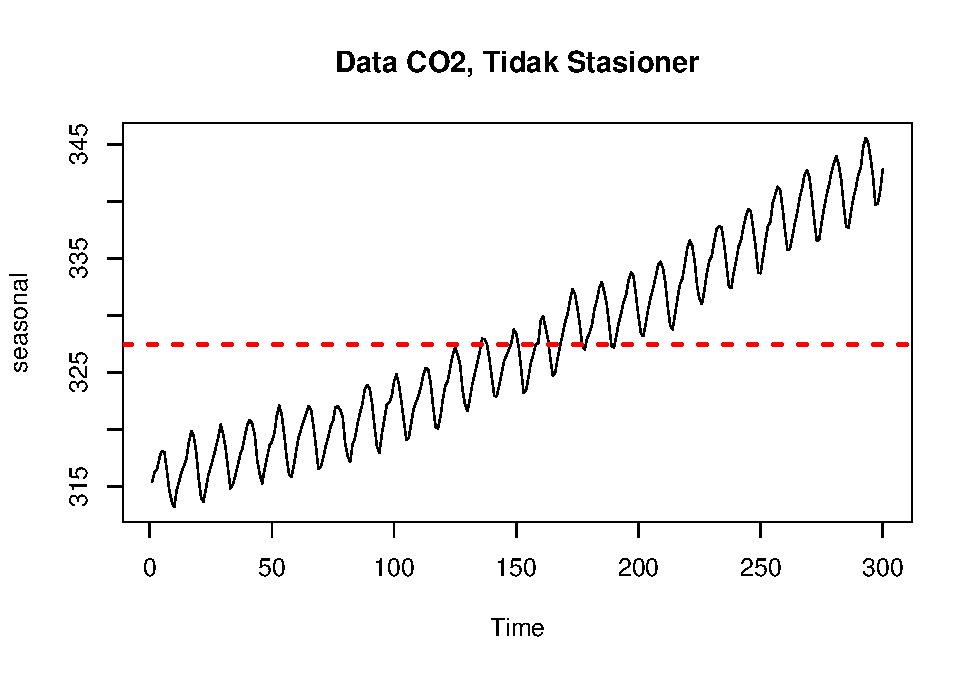
\includegraphics{_main_files/figure-latex/Contoh Plot yang Stasioner daan Tidak Stasioner-1} \end{center}

\begin{longtable}[]{@{}l@{}}
\toprule\noalign{}
Jurnal Praktikum 3 \\
\midrule\noalign{}
\endhead
\bottomrule\noalign{}
\endlastfoot
1. Berikan interpretasi anda terhadap gambar tersebut ! \\
2. Apakah data tersebar pada rataan data ? \\
3. Apakah terdapat pola tren data ? \\
\end{longtable}

\begin{Shaded}
\begin{Highlighting}[]
\CommentTok{\# Seed agar simulasi tetap sama}
\FunctionTok{set.seed}\NormalTok{(}\DecValTok{1602}\NormalTok{)}

\CommentTok{\# Membuat data Random Walk}
\NormalTok{random\_walk }\OtherTok{\textless{}{-}} \FunctionTok{arima.sim}\NormalTok{(}\AttributeTok{model =} \FunctionTok{list}\NormalTok{(}\AttributeTok{order=}\FunctionTok{c}\NormalTok{(}\DecValTok{0}\NormalTok{,}\DecValTok{1}\NormalTok{,}\DecValTok{0}\NormalTok{)),}\AttributeTok{n=}\DecValTok{300}\NormalTok{)}
\FunctionTok{plot}\NormalTok{(random\_walk, }\AttributeTok{main =} \StringTok{\textquotesingle{}Data Random Walk, Tidak Stasioner\textquotesingle{}}\NormalTok{)}
\FunctionTok{abline}\NormalTok{(}\AttributeTok{h=}\FunctionTok{mean}\NormalTok{(random\_walk),}\AttributeTok{col=}\StringTok{\textquotesingle{}red\textquotesingle{}}\NormalTok{,}\AttributeTok{lwd=}\DecValTok{2}\NormalTok{,}\AttributeTok{lty =} \DecValTok{2}\NormalTok{)}
\end{Highlighting}
\end{Shaded}

\begin{center}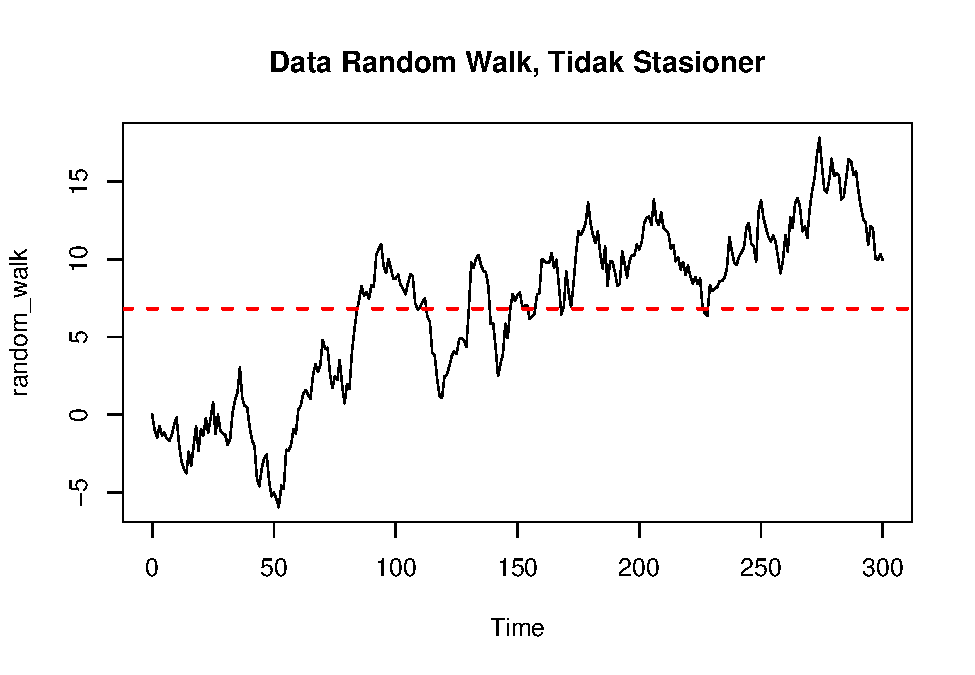
\includegraphics{_main_files/figure-latex/Contoh Plot yang Stasioner a Tidak Stasioner-1} \end{center}

\begin{longtable}[]{@{}l@{}}
\toprule\noalign{}
Jurnal Praktikum 4 \\
\midrule\noalign{}
\endhead
\bottomrule\noalign{}
\endlastfoot
1. Berikan interpretasi anda terhadap gambar tersebut ! \\
2. Apakah data tersebar pada rataan data ? \\
3. Apakah terdapat pola tren data ? \\
\end{longtable}

\hypertarget{autokorelasi}{%
\section{Autokorelasi}\label{autokorelasi}}

Misalkan proses \(\{Y_t\}\) stasioner maka korelasi antar peubah acak yang terpisah sejauh \(k\) lag waktu adalah:
\begin{align*}
\rho_k &= \text{Corr}(Y_t, Y_{t-k}) \\
&= \frac{\text{Cov}(Y_t, Y_{t-k})}{\sqrt{\text{Var}(Y_t)\text{Var}(Y_{t-k})}} \\
&= \frac{\gamma_k}{\gamma_0}, \quad k \in \mathbb{N}_0
\end{align*}
Terdapat statistik uji untuk menguji apakah nilai autokorelasi pada suatu lag ke-\(k\) signifikan atau tidak. Statistik uji tersebut adalah statistik \textbf{uji \(t_{ratio}\)} dengan
\begin{align*}
H_0 : \rho_k = 0 \\
H_1 : \rho_k \neq 0 
\end{align*}
dengan \(k \in \mathbb{N}\). Statistik hitung dari uji ini adalah:
\begin{equation}
t_{\text{ratio}} := \frac{\hat{\rho}_k}{\sqrt{\left( 1 + \sum_{i = 1}^{k - 1} \hat{\rho}_i\right)/n}} \label{eq:tratio}
\end{equation}
dengan \(n\) adalah ukuran sampel.\\
\(H_0\) akan ditolak jika \(|t_{\text{hitung}}| > Z_{1-\frac{\alpha}{2}}\) dengan \(Z_{1-\frac{\alpha}{2}}\) adalah persentil ke-(\(1-\frac{\alpha}{2}\)) dari distribusi normal baku.\\
Sedangkan statistik uji untuk menguji apakah autokorelasi dari lag pertama hingga lag ke-\(k\) signikan adalah Uji Ljung Box dengan:
\begin{align*}
H_0 &: \rho_1 = \rho_2 = \dots = \rho_k = 0 \\
H_1 &: \rho_j \neq 0, \quad \quad j \in \{1, \dots, k \} 
\end{align*}
dengan \(k \in \mathbb{N}\). Statistik hitung dari uji ini adalah:
\begin{equation}
Q(k) := n\left(n+2\right)\sum_{i=1}^k \frac{\hat{\rho}_i^2}{n-i} \label{eq:statuji}
\end{equation}
\(H_0\) ditolak jika \(Q(k) > \chi^2_{1-\alpha,k}\) dengan \(\chi^2_{1-\alpha,k}\) adalah nilai persentil \(1-\alpha\) dari distribusi \(\chi^2\) dengan derajat kebebasan \(k\).

\hypertarget{random-walk}{%
\section{Random Walk}\label{random-walk}}

Misalkan \(\varepsilon_1,\varepsilon_2, \dots\) barisan peubah acak yang berdistribusi Normal yang saling bebas dan identik dengan \(E[\varepsilon_i]=0\) dan \(\text{Var}(\varepsilon_i) =\sigma^2_\varepsilon\) untuk semua \(i\). Maka proses \emph{random walk} dapat dikonstruksi dengan persamaan berikut:
\begin{equation}
Y_t = \sum_{i=1}^t \varepsilon_i \label{eq:rw}
\end{equation}
yang dapat ditulis secara rekursif seperti berikut:
\begin{equation}
Y_t = Y_{t-1} - \varepsilon_t
\end{equation}

\hypertarget{contoh-soal}{%
\section{Contoh Soal}\label{contoh-soal}}

\begin{quote}
Unduh data berikut ini
\end{quote}

\begin{longtable}[]{@{}
  >{\raggedright\arraybackslash}p{(\columnwidth - 0\tabcolsep) * \real{1.0000}}@{}}
\toprule\noalign{}
\begin{minipage}[b]{\linewidth}\raggedright
\href{https://drive.google.com/uc?export=download\&id=1zevgGmfz87MJYn8OuIX5FEBgypR-DWnG}{TEKAN UNTUK MENGUNDUH DATA}
\end{minipage} \\
\midrule\noalign{}
\endhead
\bottomrule\noalign{}
\endlastfoot
\end{longtable}

\begin{quote}
kemudian buatlah algoritma untuk menghitung :\\
1. Rataan dari data;\\
2. Kovariansi dari data; dan\\
3. Korelasi dari data
\end{quote}

\begin{Shaded}
\begin{Highlighting}[]
\CommentTok{\# Membaca data}
\FunctionTok{library}\NormalTok{(readxl)}
\NormalTok{df }\OtherTok{\textless{}{-}} \FunctionTok{read\_excel}\NormalTok{(}\StringTok{"data.xlsx"}\NormalTok{)  }

\CommentTok{\# Membuat plot data}
\FunctionTok{plot}\NormalTok{(df}\SpecialCharTok{$}\NormalTok{Date, df}\SpecialCharTok{$}\StringTok{\textasciigrave{}}\AttributeTok{Ice Cream Sales}\StringTok{\textasciigrave{}}\NormalTok{, }\AttributeTok{type =} \StringTok{\textquotesingle{}line\textquotesingle{}}\NormalTok{, }
   \AttributeTok{xlab=} \StringTok{\textquotesingle{}Tanggal\textquotesingle{}}\NormalTok{, }\AttributeTok{ylab=} \StringTok{\textquotesingle{}Penjualan Es Krim\textquotesingle{}}\NormalTok{, }
   \AttributeTok{col =} \StringTok{\textquotesingle{}black\textquotesingle{}}\NormalTok{, }
   \AttributeTok{main =} \StringTok{\textquotesingle{}Plot Data Penjualan Es Krim\textquotesingle{}}\NormalTok{)}
\FunctionTok{abline}\NormalTok{(}\AttributeTok{h=}\FunctionTok{mean}\NormalTok{(df}\SpecialCharTok{$}\StringTok{\textasciigrave{}}\AttributeTok{Ice Cream Sales}\StringTok{\textasciigrave{}}\NormalTok{), }
     \AttributeTok{col=}\StringTok{\textquotesingle{}red\textquotesingle{}}\NormalTok{,}
     \AttributeTok{lwd=}\DecValTok{2}\NormalTok{,}\AttributeTok{lty =} \DecValTok{2}\NormalTok{)}
\end{Highlighting}
\end{Shaded}

\begin{center}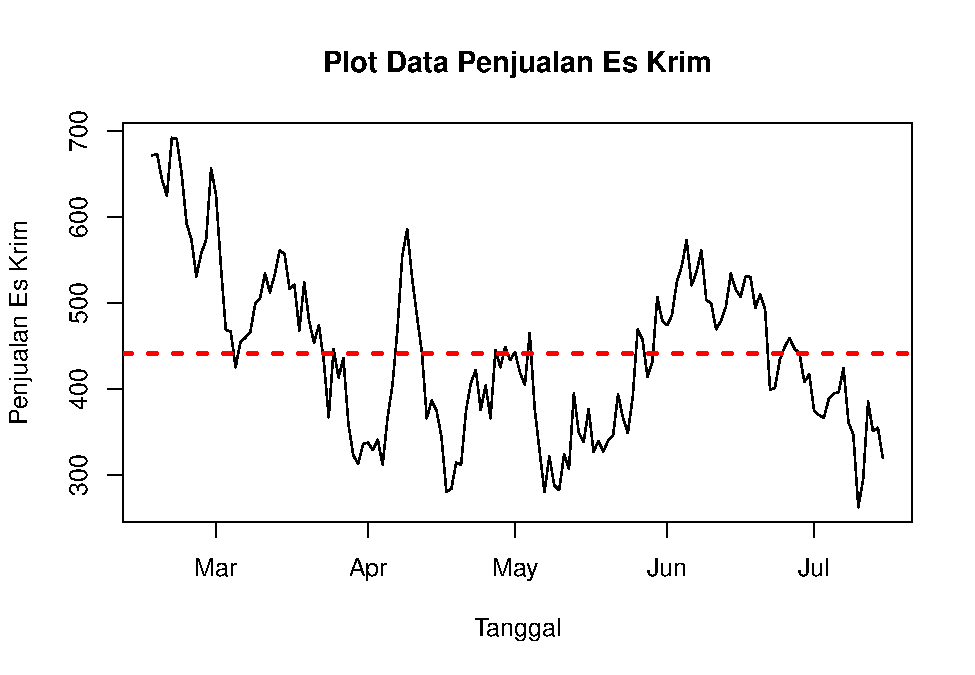
\includegraphics{_main_files/figure-latex/Contoh Soal-1} \end{center}

\begin{Shaded}
\begin{Highlighting}[]
\CommentTok{\# Algoritma menghitung rataan (boleh menggunakan sum)  }
\NormalTok{sum\_x }\OtherTok{\textless{}{-}} \FunctionTok{sum}\NormalTok{(df}\SpecialCharTok{$}\StringTok{\textasciigrave{}}\AttributeTok{Ice Cream Sales}\StringTok{\textasciigrave{}}\NormalTok{)}
\NormalTok{len }\OtherTok{\textless{}{-}} \FunctionTok{length}\NormalTok{(df}\SpecialCharTok{$}\StringTok{\textasciigrave{}}\AttributeTok{Ice Cream Sales}\StringTok{\textasciigrave{}}\NormalTok{)}
\NormalTok{rata\_x }\OtherTok{\textless{}{-}}\NormalTok{ sum\_x}\SpecialCharTok{/}\NormalTok{len}

\CommentTok{\# Algoritma menghitung kovariansi  }
\NormalTok{maxLag }\OtherTok{\textless{}{-}} \DecValTok{24}
\NormalTok{kov }\OtherTok{\textless{}{-}} \FunctionTok{rep}\NormalTok{(}\DecValTok{0}\NormalTok{, maxLag)}
\ControlFlowTok{for}\NormalTok{ (k }\ControlFlowTok{in} \DecValTok{1}\SpecialCharTok{:}\NormalTok{ maxLag) \{}
\NormalTok{x\_star }\OtherTok{\textless{}{-}}\NormalTok{ df}\SpecialCharTok{$}\StringTok{\textasciigrave{}}\AttributeTok{Ice Cream Sales}\StringTok{\textasciigrave{}}\NormalTok{[}\DecValTok{1}\SpecialCharTok{:}\NormalTok{(len}\SpecialCharTok{{-}}\NormalTok{k}\SpecialCharTok{+}\DecValTok{1}\NormalTok{)]}\SpecialCharTok{{-}}
  \FunctionTok{mean}\NormalTok{(df}\SpecialCharTok{$}\StringTok{\textasciigrave{}}\AttributeTok{Ice Cream Sales}\StringTok{\textasciigrave{}}\NormalTok{[}\DecValTok{1}\SpecialCharTok{:}\NormalTok{(len}\SpecialCharTok{{-}}\NormalTok{k}\SpecialCharTok{+}\DecValTok{1}\NormalTok{)]) }
\NormalTok{y\_star }\OtherTok{\textless{}{-}}\NormalTok{ df}\SpecialCharTok{$}\StringTok{\textasciigrave{}}\AttributeTok{Ice Cream Sales}\StringTok{\textasciigrave{}}\NormalTok{[(}\DecValTok{1}\SpecialCharTok{+}\NormalTok{k}\DecValTok{{-}1}\NormalTok{)}\SpecialCharTok{:}\NormalTok{len]}\SpecialCharTok{{-}}
  \FunctionTok{mean}\NormalTok{(df}\SpecialCharTok{$}\StringTok{\textasciigrave{}}\AttributeTok{Ice Cream Sales}\StringTok{\textasciigrave{}}\NormalTok{[(}\DecValTok{1}\SpecialCharTok{+}\NormalTok{k}\DecValTok{{-}1}\NormalTok{)}\SpecialCharTok{:}\NormalTok{len])}
\NormalTok{kov[k]  }\OtherTok{\textless{}{-}}\NormalTok{  (x\_star)}\SpecialCharTok{\%*\%}\NormalTok{(y\_star) }\SpecialCharTok{/}\NormalTok{(len)}
\NormalTok{\}}
\CommentTok{\# Algoritma menghitung korelasi}
\NormalTok{kor }\OtherTok{\textless{}{-}} \FunctionTok{rep}\NormalTok{(}\DecValTok{0}\NormalTok{, maxLag)}
\ControlFlowTok{for}\NormalTok{ (k }\ControlFlowTok{in} \DecValTok{1}\SpecialCharTok{:}\NormalTok{ maxLag) \{}
\NormalTok{x\_star }\OtherTok{\textless{}{-}}\NormalTok{ df}\SpecialCharTok{$}\StringTok{\textasciigrave{}}\AttributeTok{Ice Cream Sales}\StringTok{\textasciigrave{}}\NormalTok{[}\DecValTok{1}\SpecialCharTok{:}\NormalTok{(len}\SpecialCharTok{{-}}\NormalTok{k}\SpecialCharTok{+}\DecValTok{1}\NormalTok{)]}\SpecialCharTok{{-}}
  \FunctionTok{mean}\NormalTok{(df}\SpecialCharTok{$}\StringTok{\textasciigrave{}}\AttributeTok{Ice Cream Sales}\StringTok{\textasciigrave{}}\NormalTok{[}\DecValTok{1}\SpecialCharTok{:}\NormalTok{(len}\SpecialCharTok{{-}}\NormalTok{k}\SpecialCharTok{+}\DecValTok{1}\NormalTok{)]) }
\NormalTok{y\_star }\OtherTok{\textless{}{-}}\NormalTok{ df}\SpecialCharTok{$}\StringTok{\textasciigrave{}}\AttributeTok{Ice Cream Sales}\StringTok{\textasciigrave{}}\NormalTok{[k}\SpecialCharTok{:}\NormalTok{len]}\SpecialCharTok{{-}}
  \FunctionTok{mean}\NormalTok{(df}\SpecialCharTok{$}\StringTok{\textasciigrave{}}\AttributeTok{Ice Cream Sales}\StringTok{\textasciigrave{}}\NormalTok{[k}\SpecialCharTok{:}\NormalTok{len])}
\NormalTok{penyebut }\OtherTok{\textless{}{-}} \FunctionTok{sqrt}\NormalTok{((x\_star}\SpecialCharTok{\%*\%}\NormalTok{x\_star)}\SpecialCharTok{*}\NormalTok{(y\_star}\SpecialCharTok{\%*\%}\NormalTok{y\_star))}
\NormalTok{kor[k]  }\OtherTok{\textless{}{-}}\NormalTok{  x\_star}\SpecialCharTok{\%*\%}\NormalTok{y\_star}\SpecialCharTok{/}\NormalTok{penyebut}
\NormalTok{\}}
\end{Highlighting}
\end{Shaded}

Penjelasan lebih lanjut :
Persamaan kovariansi dapat ditulis sebagai berikut :
\begin{equation}
\hat{\gamma}_{XY} = \frac{\sum_{i=1}^n (x_i - \bar{x})(y_i - \bar{y})}{n} = \frac{1}{n}(\vec{x}^* \cdot \vec{y}^*) 
\end{equation}
dengan \(\vec{x}^* = (x_1 - \bar{x}, \dots, x_n - \bar{x})^T\) dan \(\vec{y}^* = (y_1 - \bar{y}, \dots, y_n - \bar{y})^T\).\\
Sedangkan persamaan korelasi dapat ditulis sebagai berikut
\begin{equation}
\hat{\rho}_{XY} = \frac{\sum_{i=1}^n (x_i - \bar{x})(y_i - \bar{y})}{\sqrt{\sum_{i=1}^n (x_i - \bar{x})^2\sum_{i=1}^n(y_i - \bar{y})^2}} = \frac{1}{\sqrt{(\vec{x}^{*^T}\cdot \vec{x}^*)(\vec{y}^{*^T}\cdot \vec{y}^{*})}}(\vec{x}^* \cdot \vec{y}^*) 
\end{equation}\\
Catatan :
Perhatikan bahwa terdapat kovariansi dan variansi sampel dan populasi. Untuk algoritma menghitung kovariansi sampel dan variansi sampel diserahkan kepada pembaca.

\hypertarget{model-deret-waktu-stasioner}{%
\chapter{Model Deret Waktu Stasioner}\label{model-deret-waktu-stasioner}}

Pada bab ini akan dipelajari perilaku umum dari ACF dan PACF untuk menentukan orde pada model deret waktu ARMA yang akan digunakan. Dua jenis perilaku umum yang ditunjukkan adalah \textbf{tails off} dan \textbf{cuts off}.\\

\begin{figure}

{\centering 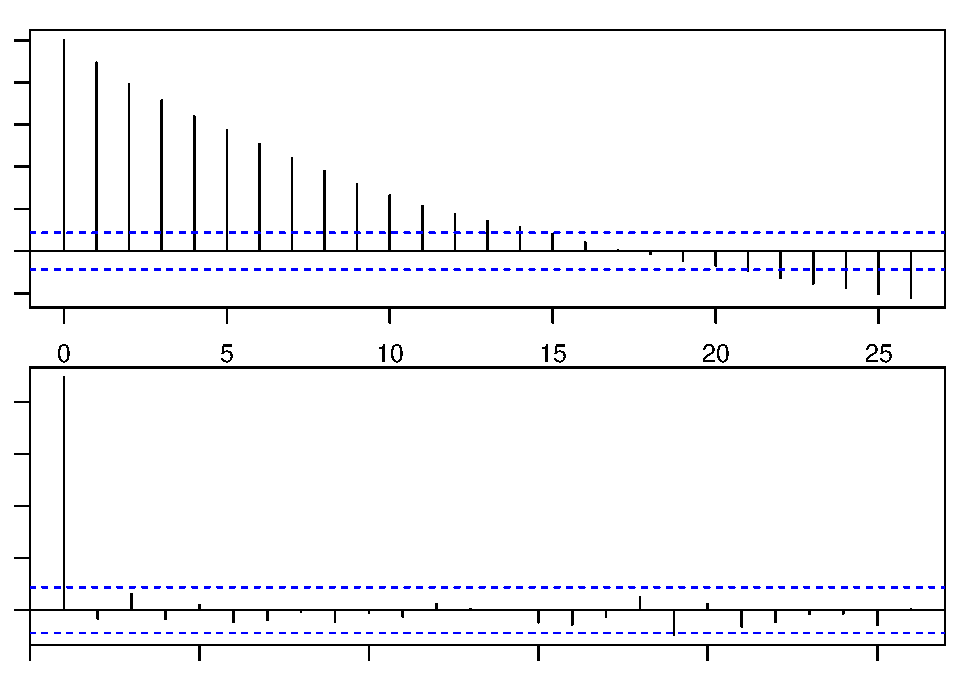
\includegraphics{_main_files/figure-latex/unnamed-chunk-1-1} 

}

\caption{*Tails off (gambar atas) dan Cuts Off (gambar bawah)*}\label{fig:unnamed-chunk-1}
\end{figure}

Berikut adalah persamaan autokorelasi sampel :
\begin{align*}
\hat{\rho}_k &= \frac{\gamma_k}{\gamma_0} \\
&= \frac{\sum_{t=1}^{n-k}(y_t - \bar{y})(y_{t+k} - \bar{y})}{\sum_{t=1}^n(y_t - \bar{y})^2} \quad k \in \mathbb{N}
\end{align*}
Sedangkan untuk persamaan autokorelasi parsial sampel adalah sebagai berikut :\\
\begin{align*}
\hat{\phi}_{ij} = \begin{cases}
\hat{\rho}_1, \quad i = j = 1 \\
\frac{\hat{\rho}_k - \sum_{j=1}^{k-1} \hat{\phi}_{k-1,j}\hat{\rho}_{k-j}}{1- \sum_{j=1}^{k-1} \hat{\phi}_{k-1,j}\hat{\rho}_{j}}, \quad k = 2,3,4,\dots \\
\hat{\phi}_{k-1,j} - \hat{\phi}_{k,k}\hat{\phi}_{k-1,k-j}, \quad j \in \mathbb{N}
\end{cases}
\end{align*}
Perilaku umum dari ACF dan PACF untuk model ARMA.

\begin{longtable}[]{@{}
  >{\raggedright\arraybackslash}p{(\columnwidth - 6\tabcolsep) * \real{0.1210}}
  >{\raggedright\arraybackslash}p{(\columnwidth - 6\tabcolsep) * \real{0.2823}}
  >{\raggedright\arraybackslash}p{(\columnwidth - 6\tabcolsep) * \real{0.2823}}
  >{\raggedright\arraybackslash}p{(\columnwidth - 6\tabcolsep) * \real{0.3145}}@{}}
\toprule\noalign{}
\begin{minipage}[b]{\linewidth}\raggedright
\end{minipage} & \begin{minipage}[b]{\linewidth}\raggedright
AR\((p)\)
\end{minipage} & \begin{minipage}[b]{\linewidth}\raggedright
MA\((q)\)
\end{minipage} & \begin{minipage}[b]{\linewidth}\raggedright
ARMA\((p,q)\)
\end{minipage} \\
\midrule\noalign{}
\endhead
\bottomrule\noalign{}
\endlastfoot
ACF & \emph{Tails off} & \emph{Cuts off} setelah lag ke-\(q\) & \emph{Tails off} setelah lag ke-\(q\) \\
PACF & \emph{Cuts off} setelah lag ke-\(p\) & \emph{Tails off} & \emph{Tails off} setelah lag ke-\(p\) \\
\end{longtable}

Model deret waktu umum yang sering digunakan adalah model regresi diri (\emph{Autoregressive}), dinotasikan AR, model rataan bergerak (\emph{Moving Average}), dinotasikan MA, dan model campuran regresi diri dan rataan bergerak (\emph{Autoregressive Moving Average}), dinotasikan ARMA.

\hypertarget{moving-average-ma}{%
\section{Moving Average (MA)}\label{moving-average-ma}}

Misalkan \(Y_t=(Y_1,Y_2,…,Y_n )\), jika proses \(\{Y_t\}\) mengikuti proses MA dengan orde \(q\) maka dapat dinyatakan dengan persamaan berikut
\begin{equation}
Y_t=\varepsilon_t - \theta_1 \varepsilon_{t-1}-\theta_2 \varepsilon_{t-2}-\dots-\theta_q \varepsilon_{t-q}
\end{equation}
Misalkan \(Y_t\) mengikuti proses MA(1) maka dapat dinyatakan dengan persamaan berikut
\begin{equation}
Y_t=\varepsilon_t - \theta_1 \varepsilon_{t-1}
\end{equation}
Karena \(\varepsilon_t\sim \text{Normal}(0,\sigma^2_\varepsilon)\), maka \(E[Y_t]=0\) dan \(\text{Var}(Y_t)=(1+\theta^2)\sigma_\varepsilon^2\) (Bukti diserahkan kepada pembaca sebagai latihan).\\
sedangkan untuk kovariansi dari model MA dapat diperoleh sebagai berikut\\
\begin{align*}
\text{Cov}(Y_t,Y_{t-1}) &=\text{Cov}(\varepsilon_t-\theta_1 \varepsilon_{t-1}, \varepsilon_{t-1}-\theta_1 \varepsilon_{t-2}) \\
&=-\theta_1 \text{Cov}(\varepsilon_{t-1},\varepsilon_{t-1}) \quad (\text{Mengapa?}) \\
&=-\theta_1 \sigma_\varepsilon^2
\end{align*}
dan
\begin{align*}
\text{Cov}(Y_t,Y_{t-2})&=\text{Cov}(\varepsilon_t - \theta_1 \varepsilon_{t-1},\varepsilon_{t-2}-\theta_1\varepsilon_{t-3}) \\ 
&= 0 \quad \text{(Mengapa?)}
\end{align*}
Sehingga fungsi autokovariansi untuk model MA(1) adalah
\begin{align*}
\gamma_k = \begin{cases}
(1+\theta_1^2)\sigma^2_\varepsilon, \quad &k =0 \\
-\theta_1 \sigma^2_\varepsilon, \quad &k = 1 \\ 
0, \quad &k > 1
\end{cases}
\end{align*}
dan fungsi autokorelasinya adalah
\begin{align*}
\rho_k = \begin{cases}
1, \quad &k =0 \\
\frac{-\theta_1}{1+\theta^2_1}, \quad &k = 1 \\ 
0, \quad &k >1
\end{cases}
\end{align*}
Untuk membuat simulasi model MA(1) dapat menggunakan kode berikut :

\begin{Shaded}
\begin{Highlighting}[]
\NormalTok{n\_sim }\OtherTok{\textless{}{-}} \DecValTok{150} \CommentTok{\# Banyak data }
\NormalTok{theta }\OtherTok{\textless{}{-}} \SpecialCharTok{{-}}\FloatTok{0.8} \CommentTok{\# Nilai dari theta\_1}
\NormalTok{simulasi\_ar }\OtherTok{\textless{}{-}} \FunctionTok{arima.sim}\NormalTok{(}\AttributeTok{model =} \FunctionTok{list}\NormalTok{(}\FunctionTok{c}\NormalTok{(}\DecValTok{0}\NormalTok{,}\DecValTok{0}\NormalTok{,}\DecValTok{1}\NormalTok{), }\AttributeTok{ma =}\NormalTok{ theta), }
                       \AttributeTok{n =}\NormalTok{ n\_sim)}
\FunctionTok{plot}\NormalTok{(simulasi\_ar, }\AttributeTok{main =} \StringTok{\textquotesingle{}Grafik Data MA(1)\textquotesingle{}}\NormalTok{)}
\end{Highlighting}
\end{Shaded}

\begin{center}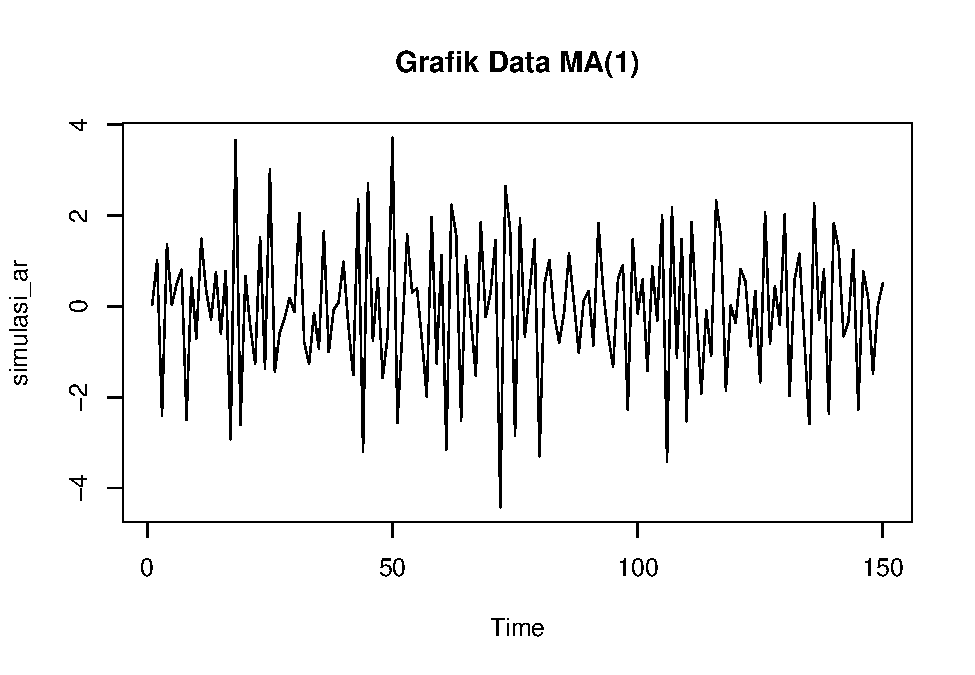
\includegraphics{_main_files/figure-latex/Model MA-1} \end{center}

\begin{Shaded}
\begin{Highlighting}[]
\FunctionTok{acf}\NormalTok{(simulasi\_ar, }\AttributeTok{main =} \StringTok{\textquotesingle{}Grafik ACF Data MA(1)\textquotesingle{}}\NormalTok{, }
  \AttributeTok{lag.max =} \DecValTok{36}\NormalTok{)}
\end{Highlighting}
\end{Shaded}

\begin{center}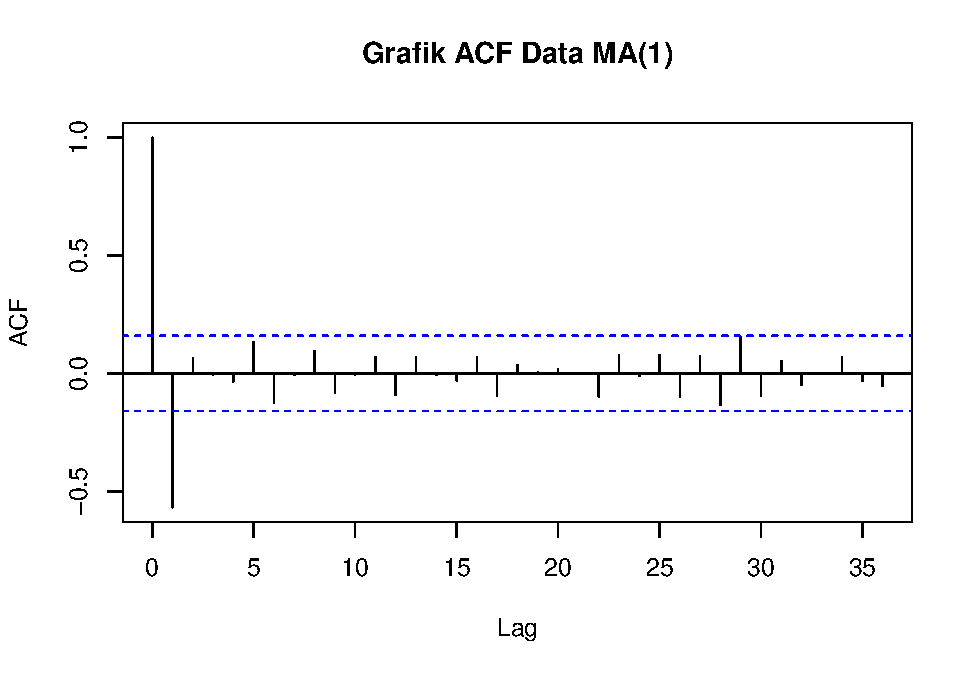
\includegraphics{_main_files/figure-latex/Model MA-2} \end{center}

\begin{Shaded}
\begin{Highlighting}[]
\FunctionTok{pacf}\NormalTok{(simulasi\_ar, }\AttributeTok{main =} \StringTok{\textquotesingle{}Grafik PACF Data MA(1)\textquotesingle{}}\NormalTok{, }
  \AttributeTok{lag.max =} \DecValTok{36}\NormalTok{)}
\end{Highlighting}
\end{Shaded}

\begin{center}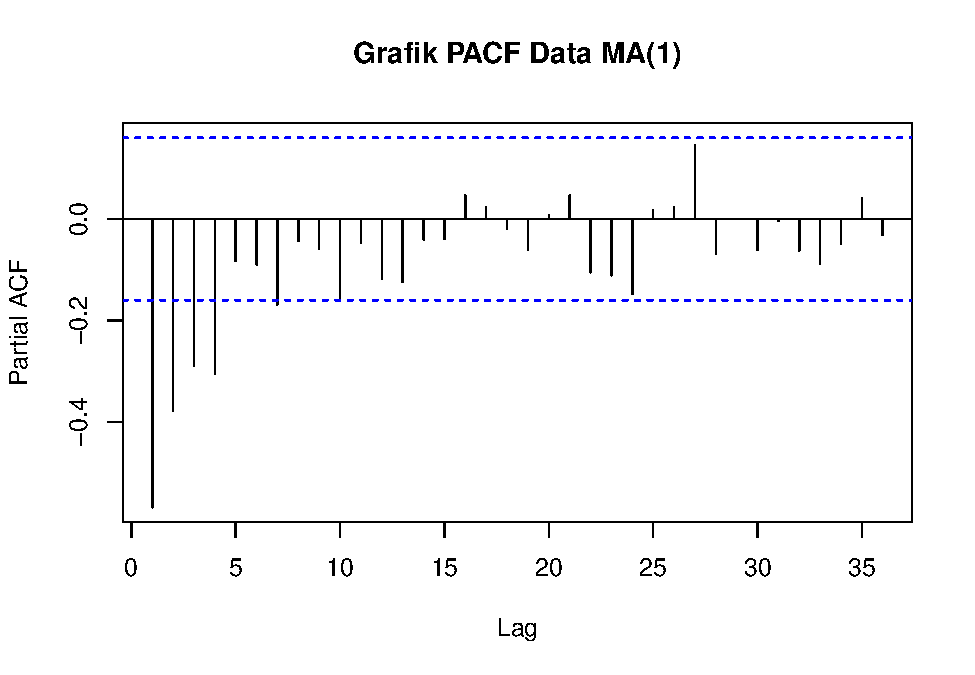
\includegraphics{_main_files/figure-latex/Model MA-3} \end{center}
\begin{jp}{}{}
\begin{enumerate}
\item Berikan interpretasi anda mengenai grafik tersebut !  
\item Apakah data tersebar pada rataan data ?  
\item Apakah terdapat pola tren data ?
\end{enumerate}
\end{jp}

\begin{Shaded}
\begin{Highlighting}[]
\FunctionTok{acf}\NormalTok{(simulasi\_ar, }\AttributeTok{main =} \StringTok{\textquotesingle{}Grafik ACF Data MA(1)\textquotesingle{}}\NormalTok{, }
  \AttributeTok{lag.max =} \DecValTok{36}\NormalTok{)}
\end{Highlighting}
\end{Shaded}

\begin{center}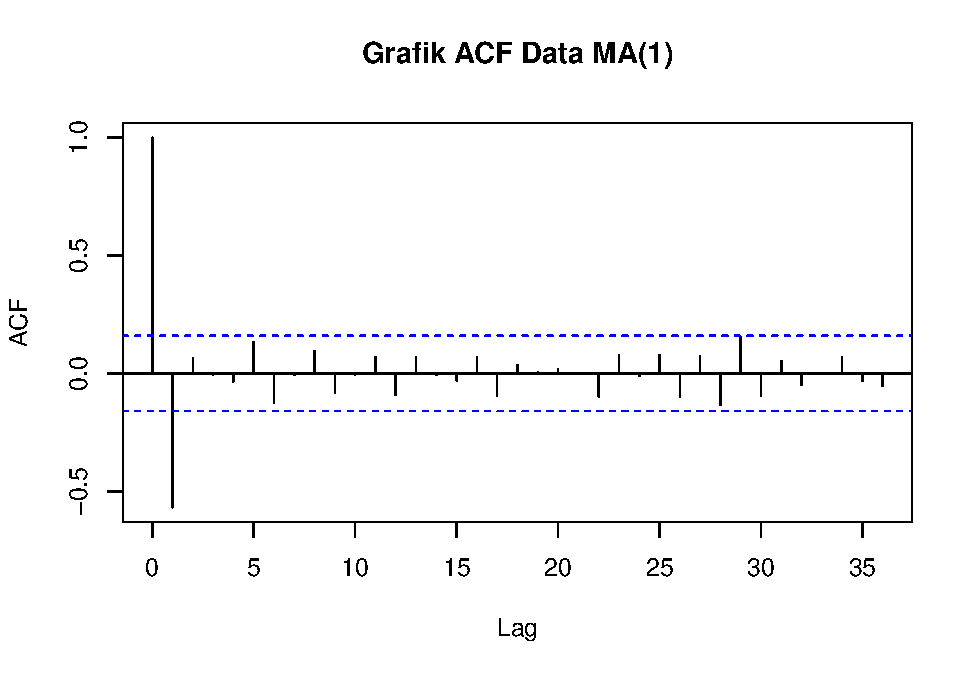
\includegraphics{_main_files/figure-latex/acf MA-1} \end{center}
\begin{jp}{}{}
\begin{enumerate}
\item Berikan interpretasi anda mengenai grafik tersebut !  
\item Apakah ACF berprilaku sesuai dengan model MA ? 
\item Apakah data tersebut masih cocok dimodelkan dengan model MA(1) ? Berikan alasan anda !
\end{enumerate}
\end{jp}

\begin{Shaded}
\begin{Highlighting}[]
\FunctionTok{pacf}\NormalTok{(simulasi\_ar, }\AttributeTok{main =} \StringTok{\textquotesingle{}Grafik PACF Data MA(1)\textquotesingle{}}\NormalTok{, }
  \AttributeTok{lag.max =} \DecValTok{36}\NormalTok{)}
\end{Highlighting}
\end{Shaded}

\begin{center}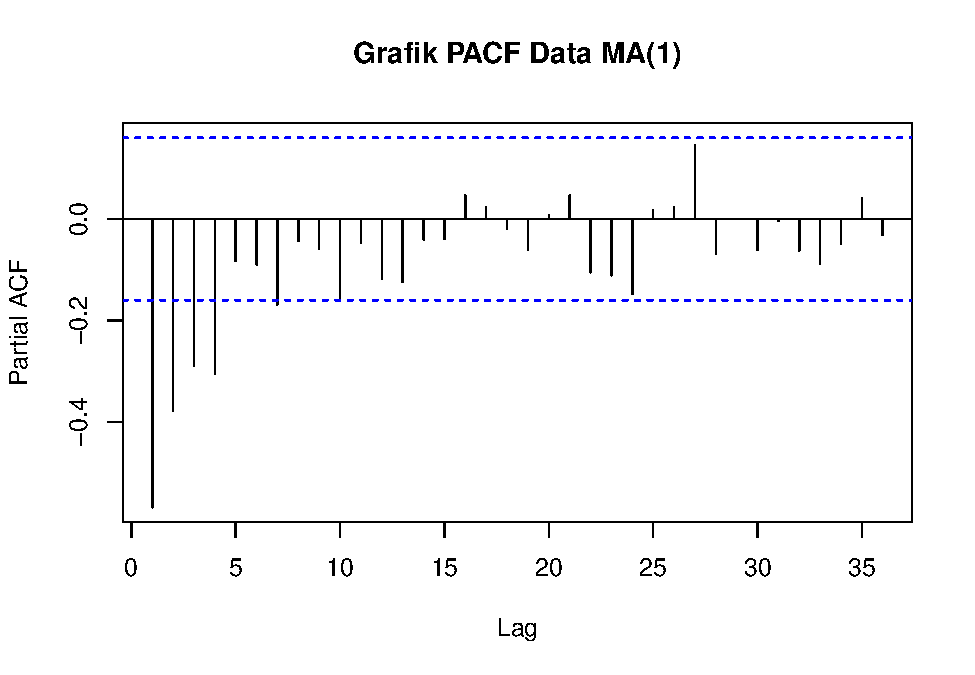
\includegraphics{_main_files/figure-latex/pacf MA-1} \end{center}
\begin{jp}{}{}
\begin{enumerate}
\item Berikan interpretasi anda mengenai grafik tersebut !  
\item Apakah PACF berprilaku sesuai dengan model MA ?
\item Apakah data tersebut masih cocok dimodelkan dengan model MA(1) ? Berikan alasan anda !
\item Ulangi langkah-langkah di atas dengan mengganti nilai variabel theta dan n\_sim!
\end{enumerate}
\end{jp}

Catatan: Nilai variabel theta dibuat negatif karena bahasa pemrograman R mendefinisikan model MA (\(q\)) sebagai:
\begin{equation}
Y_t=\varepsilon_t + \theta_1 \varepsilon_{t-1} + \theta_2 \varepsilon_{t-2} + \dots + \theta_q \varepsilon_{t-q}
\end{equation}

\hypertarget{autoregressive-ar}{%
\section{Autoregressive (AR)}\label{autoregressive-ar}}

Misalkan \(Y_t=(Y_1,Y_2,…,Y_n )\), jika proses \(\{Y_t\}\) mengikuti proses Autoregressive (AR) dengan orde \(p\) maka dapat dinyatakan dengan persamaan berikut
\begin{equation}
Y_t=\phi_1 Y_{t-1}+\phi_2 Y_{t-2}+\dots+\phi_p Y_{t-p}+\varepsilon_t
\end{equation}
Interpretasi dari persamaan di atas adalah : nilai saat ini dari deret waktu \(Y_t\) adalah kombinasi linier dari \(p\) nilai dirinya di masa lalu ditambah dengan galat, \(\varepsilon_t\)
Misalkan proses \(\{Y_t\}\) terpusat, \(Y_t\) mengikuti proses AR(1) maka dapat dinyatakan dengan persamaan berikut
\begin{equation}
Y_t=\phi_1 Y_{t-1}+\varepsilon_t
\end{equation}
Karena \(\varepsilon_t\sim \text{Normal}(0,\sigma^2_\varepsilon)\), maka \(E[Y_t]= 0\) dan \(\text{Var}(Y_t)=\frac{\sigma_\varepsilon^2}{1-\phi_1^2}\) (Bukti diserahkan kepada pembaca sebagai latihan)
sedangkan untuk kovariansinya dapat diperoleh
\begin{align*}
\text{Cov}(Y_t,Y_{t-1}) &=\text{Cov}(\phi_1 Y_{t-1}+\varepsilon_t,Y_{t-1} ) \\
&=\phi_1 \text{Cov}(Y_{t-1},Y_{t-1})+\text{Cov}(\varepsilon_{t},Y_{t-1} ) \\
&=\phi_1 \gamma_0
\end{align*}\\
dan
\begin{align*}
\text{Cov}(Y_t,Y_{t-2})&=\text{Cov}(\phi_1  Y_{t-1}+\varepsilon_t, Y_{t-2}) \\ 
&= \text{Cov}(\phi_1  (\phi_1Y_{t-2}+\varepsilon_{t-1})+\varepsilon_t, Y_{t-2}) \\ 
&= \text{Cov}(\phi_1^2 Y_{t-2},Y_{t-2}) + \text{Cov}(\phi_1\varepsilon_{t-1}),Y_{t-2}) + \text{Cov}(\varepsilon_t,Y_{t-2}) \\
&=\phi_1^2\gamma_0
\end{align*}
sehingga fungsi autokovariansi untuk model AR(1) adalah
\begin{align*}
\gamma_k = \frac{\phi_1^k \sigma_\varepsilon^2}{1-\phi_1^2}, \quad k \geq 0 
\end{align*}
dan fungsi autokorelasinya adalah
\begin{align*}
\rho_k = \frac{\gamma_k}{\gamma_0} = \phi_1^k \quad k \geq 0
\end{align*}
Untuk membuat simulasi model AR(1) dapat menggunakan kode berikut :

\begin{Shaded}
\begin{Highlighting}[]
\NormalTok{n\_sim }\OtherTok{\textless{}{-}} \DecValTok{150} \CommentTok{\# Banyak data }
\NormalTok{phi }\OtherTok{\textless{}{-}} \FloatTok{0.2} \CommentTok{\# Nilai dari phi\_1 }
\NormalTok{simulasi\_ar }\OtherTok{\textless{}{-}} \FunctionTok{arima.sim}\NormalTok{(}\AttributeTok{model =} \FunctionTok{list}\NormalTok{(}\FunctionTok{c}\NormalTok{(}\DecValTok{1}\NormalTok{,}\DecValTok{0}\NormalTok{,}\DecValTok{0}\NormalTok{), }\AttributeTok{ar =}\NormalTok{ phi), }
                       \AttributeTok{n =}\NormalTok{ n\_sim)}
\FunctionTok{plot}\NormalTok{(simulasi\_ar, }\AttributeTok{main =} \StringTok{\textquotesingle{}Grafik Data AR(1)\textquotesingle{}}\NormalTok{)}
\end{Highlighting}
\end{Shaded}

\begin{center}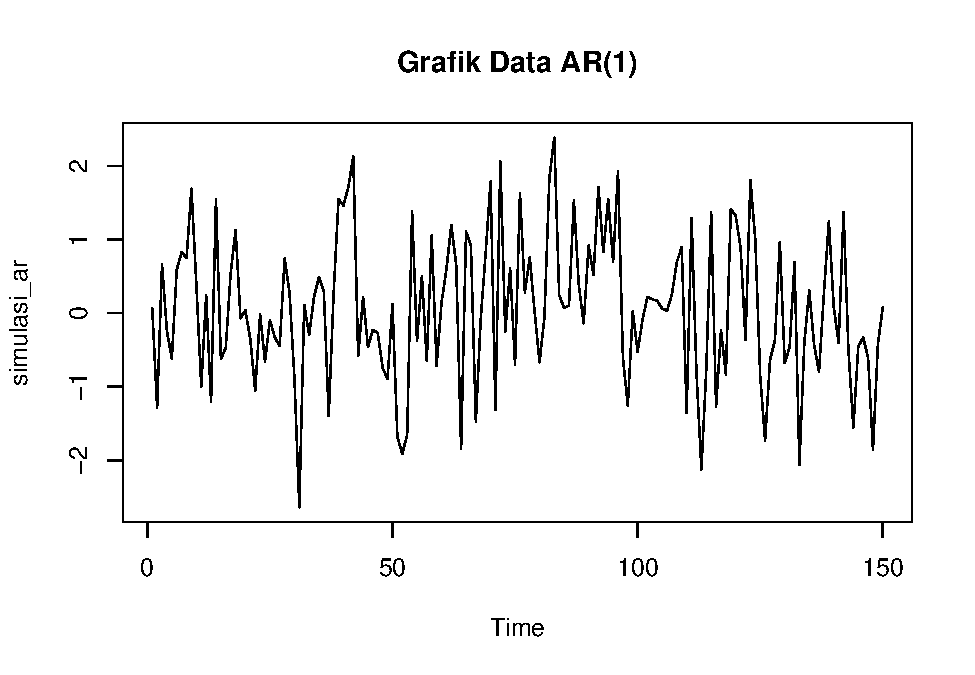
\includegraphics{_main_files/figure-latex/Model AR-1} \end{center}
\begin{jp}{}{}
\begin{enumerate}
\item Berikan interpretasi anda mengenai grafik tersebut !  
\item Apakah data tersebar pada rataan data ?  
\item Apakah terdapat pola tren data ?
\end{enumerate}
\end{jp}

\begin{Shaded}
\begin{Highlighting}[]
\FunctionTok{acf}\NormalTok{(simulasi\_ar, }\AttributeTok{main =} \StringTok{\textquotesingle{}Grafik ACF Data AR(1)\textquotesingle{}}\NormalTok{, }
  \AttributeTok{lag.max =} \DecValTok{36}\NormalTok{)}
\end{Highlighting}
\end{Shaded}

\begin{center}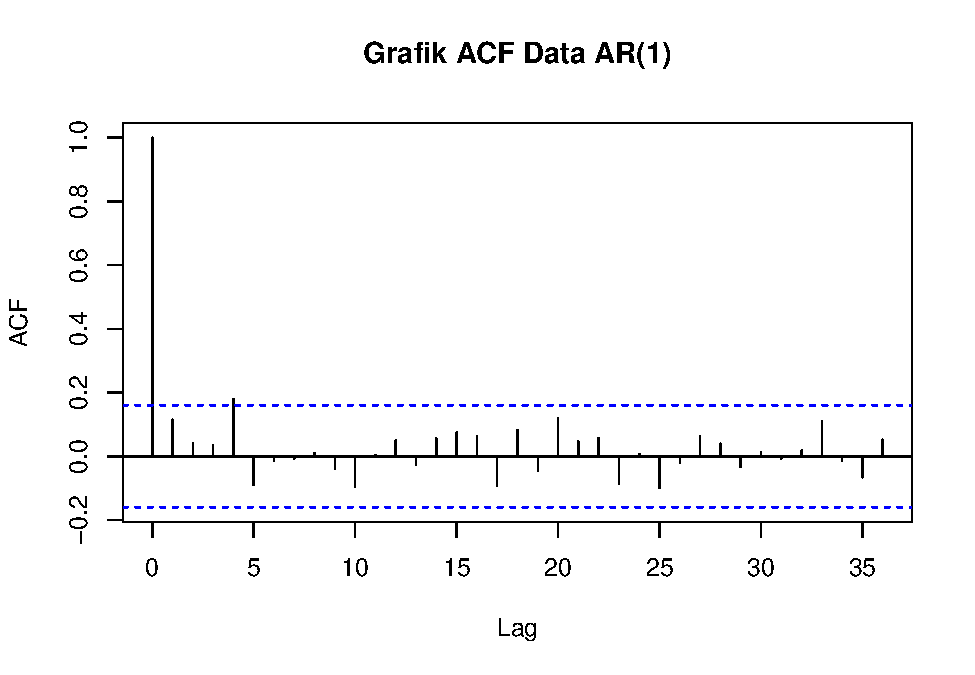
\includegraphics{_main_files/figure-latex/acf AR-1} \end{center}
\begin{jp}{}{}
\begin{enumerate}
\item Berikan interpretasi anda mengenai grafik tersebut !  
\item Apakah ACF berprilaku sesuai dengan model AR (1)?
\end{enumerate}
\end{jp}

\begin{Shaded}
\begin{Highlighting}[]
\FunctionTok{pacf}\NormalTok{(simulasi\_ar, }\AttributeTok{main =} \StringTok{\textquotesingle{}Grafik PACF Data AR(1)\textquotesingle{}}\NormalTok{, }
  \AttributeTok{lag.max =} \DecValTok{36}\NormalTok{)}
\end{Highlighting}
\end{Shaded}

\begin{center}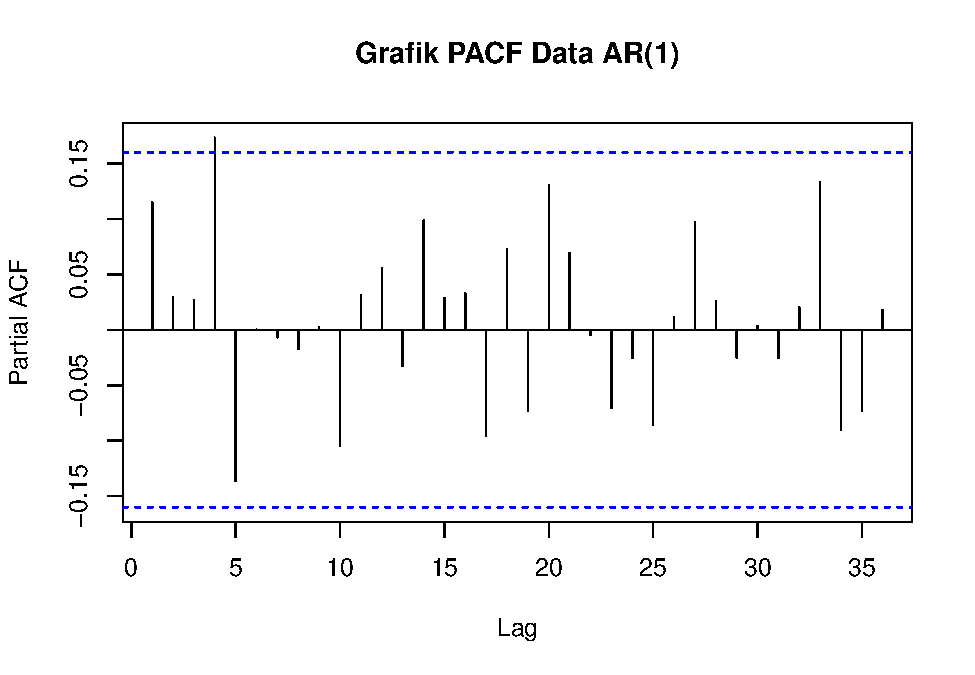
\includegraphics{_main_files/figure-latex/pacf AR-1} \end{center}

Interpretasi Gambar :

\begin{jp}{}{}
\begin{enumerate}
\item Berikan interpretasi anda mengenai grafik tersebut !  
\item Apakah PACF berprilaku sesuai dengan model AR (1)?
\item Apakah data tersebut masih cocok dimodelkan dengan model AR(1) ?
\item Ulangi langkah di atas dengan memvariasikan nilai variabel phi dan n\_sim !
\end{enumerate}
\end{jp}

\hypertarget{autoregressive-moving-average-arma}{%
\section{Autoregressive Moving Average (ARMA)}\label{autoregressive-moving-average-arma}}

Misalkan \(Y_t=(Y_1,Y_2,…,Y_n )\), jika proses \(Y_t\) mengikuti proses ARMA dengan orde \((p,q)\) maka dapat dinyatakan dengan persamaan berikut
\begin{equation}
Y_t=\phi_1 Y_{t-1}+\phi_2 Y_{t-2}+\dots+\phi_p Y_{t-p}+\varepsilon_{t}-\theta_1 \varepsilon_{t-1}-\theta_2 \varepsilon_{t-2}-\dots -\theta_q \varepsilon_{t-q}
\end{equation}
(Persamaan umum untuk \(E[Y_t]\) dan \(\text{Var}(Y_t)\) dari proses ARMA (1,1) diserahkan kepada pembaca)\\
Untuk membuat simulasi model ARMA(1,1) dapat menggunakan kode berikut :

\begin{Shaded}
\begin{Highlighting}[]
\NormalTok{n\_sim }\OtherTok{\textless{}{-}} \DecValTok{150} \CommentTok{\# Banyak data    }
\NormalTok{theta }\OtherTok{\textless{}{-}} \SpecialCharTok{{-}}\FloatTok{0.3} \CommentTok{\# Nilai dari theta\_1}
\NormalTok{phi }\OtherTok{\textless{}{-}} \FloatTok{0.2} \CommentTok{\# Nilai dari phi\_1 }
\NormalTok{simulasi\_ar }\OtherTok{\textless{}{-}} \FunctionTok{arima.sim}\NormalTok{(}\AttributeTok{model =} \FunctionTok{list}\NormalTok{(}\FunctionTok{c}\NormalTok{(}\DecValTok{1}\NormalTok{,}\DecValTok{0}\NormalTok{,}\DecValTok{1}\NormalTok{), }\AttributeTok{ar =}\NormalTok{ phi, }\AttributeTok{ma =}\NormalTok{ theta), }
                       \AttributeTok{n =}\NormalTok{ n\_sim)}
\FunctionTok{plot}\NormalTok{(simulasi\_ar, }\AttributeTok{main =} \StringTok{\textquotesingle{}Grafik Data ARMA(1,1)\textquotesingle{}}\NormalTok{)}
\end{Highlighting}
\end{Shaded}

\begin{center}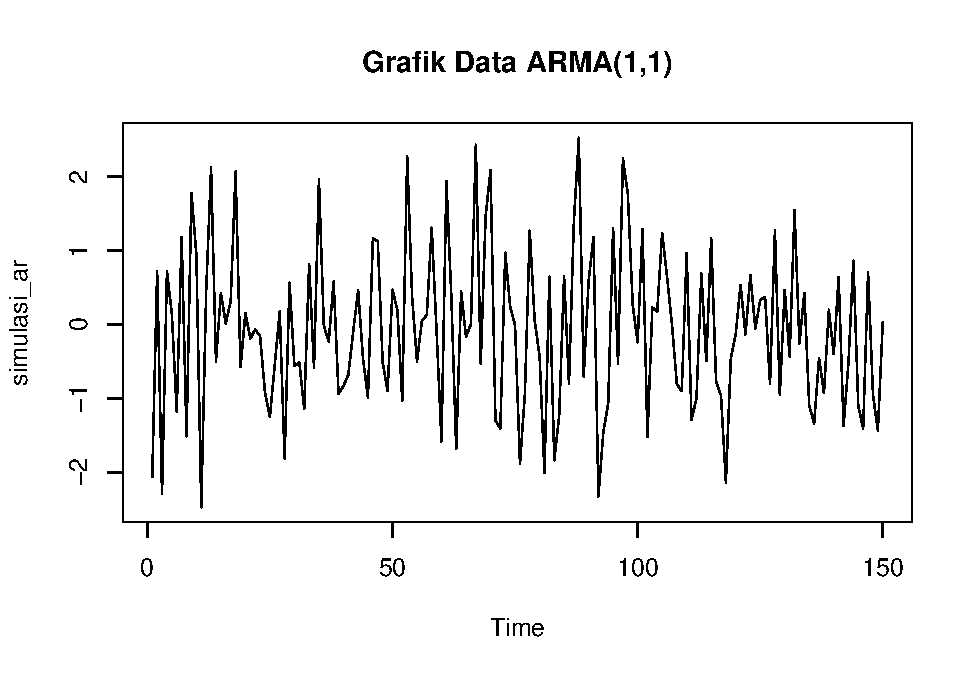
\includegraphics{_main_files/figure-latex/Model ARMA-1} \end{center}
\begin{jp}{}{}
\begin{enumerate}
\item Berikan interpretasi anda mengenai grafik tersebut !  
\item Apakah data tersebar pada rataan data ?  
\item Apakah terdapat pola tren data ?
\end{enumerate}
\end{jp}

\begin{Shaded}
\begin{Highlighting}[]
\FunctionTok{acf}\NormalTok{(simulasi\_ar, }\AttributeTok{main =} \StringTok{\textquotesingle{}Grafik ACF Data ARMA(1,1)\textquotesingle{}}\NormalTok{, }
  \AttributeTok{lag.max =} \DecValTok{36}\NormalTok{)}
\end{Highlighting}
\end{Shaded}

\begin{center}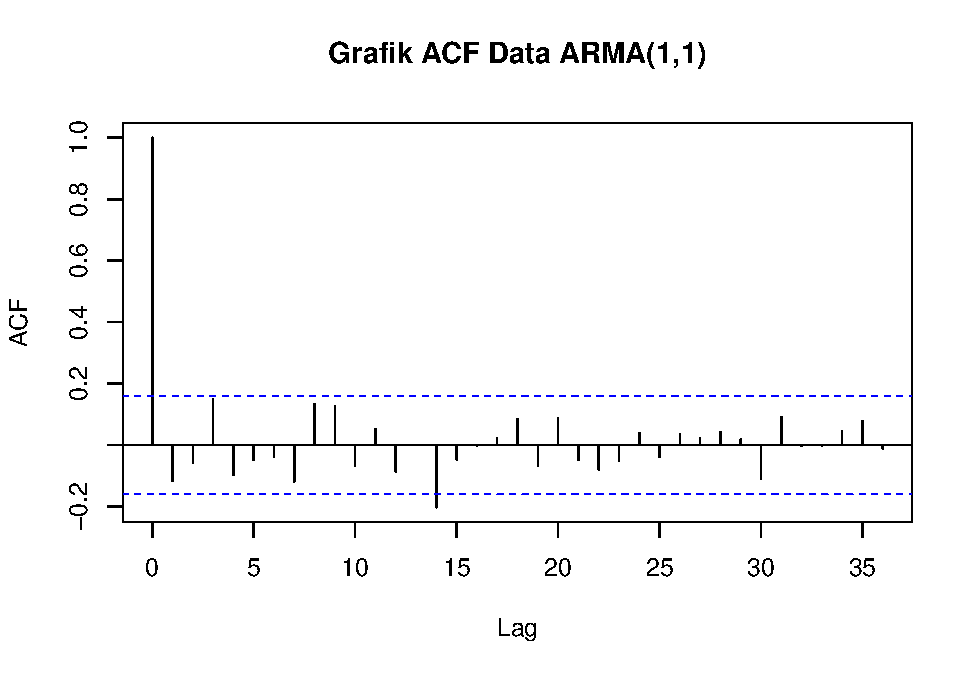
\includegraphics{_main_files/figure-latex/acf ARMA-1} \end{center}
\begin{jp}{}{}
\begin{enumerate}
\item Berikan interpretasi anda mengenai grafik tersebut !  
\item Apakah ACF berprilaku sesuai dengan model ARMA (1,1)?
\item Apakah data tersebut masih cocok dimodelkan dengan model ARMA(1,1) ?
\end{enumerate}
\end{jp}

\begin{Shaded}
\begin{Highlighting}[]
\FunctionTok{pacf}\NormalTok{(simulasi\_ar, }\AttributeTok{main =} \StringTok{\textquotesingle{}Grafik PACF Data ARMA(1,1)\textquotesingle{}}\NormalTok{, }
  \AttributeTok{lag.max =} \DecValTok{36}\NormalTok{)}
\end{Highlighting}
\end{Shaded}

\begin{center}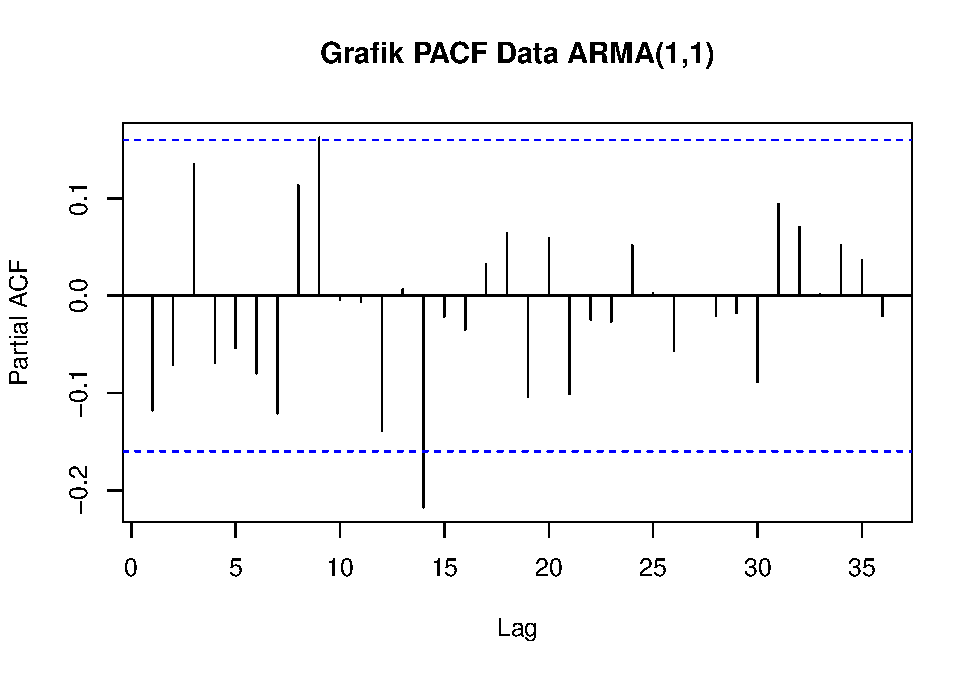
\includegraphics{_main_files/figure-latex/pacf ARMA-1} \end{center}
\begin{jp}{}{}
\begin{enumerate}
\item Berikan interpretasi anda mengenai grafik tersebut !  
\item Apakah PACF berprilaku sesuai dengan model ARMA (1,1)?
\item Apakah data tersebut masih cocok dimodelkan dengan model ARMA(1,1) ?
\end{enumerate}
\end{jp}

\hypertarget{simulasi-data-manual}{%
\section{Simulasi Data Manual}\label{simulasi-data-manual}}

Misal proses \(\{Y_t\}\) mengikuti model ARMA (1,1) maka persamaannya adalah :
\begin{equation}
Y_t=\phi_1 Y_{t-1}+\varepsilon_{t}-\theta_1 \varepsilon_{t-1}
\end{equation}

\begin{Shaded}
\begin{Highlighting}[]
\NormalTok{n\_sim }\OtherTok{\textless{}{-}} \DecValTok{100} \CommentTok{\# Banyak Data  }
\NormalTok{phi }\OtherTok{\textless{}{-}} \FloatTok{0.8} \CommentTok{\# Nilai dari phi\_1 }
\NormalTok{theta }\OtherTok{\textless{}{-}} \SpecialCharTok{{-}}\FloatTok{0.5} \CommentTok{\# Nilai dari theta\_1}
\NormalTok{sig }\OtherTok{\textless{}{-}} \DecValTok{16} \CommentTok{\# Besar standar deviasi error  }
\NormalTok{Y }\OtherTok{\textless{}{-}} \FunctionTok{c}\NormalTok{(}\FunctionTok{rep}\NormalTok{(}\DecValTok{0}\NormalTok{, }\CommentTok{\#Nilai awal}
\NormalTok{         n\_sim)) }\CommentTok{\# Membuat array / vektor data  }
\NormalTok{e }\OtherTok{\textless{}{-}} \FunctionTok{rnorm}\NormalTok{(}\AttributeTok{n =}\NormalTok{ n\_sim,}
         \AttributeTok{mean =} \DecValTok{0}\NormalTok{, }
         \AttributeTok{sd =}\NormalTok{ sig) }\CommentTok{\# Membuat galat}
\ControlFlowTok{for}\NormalTok{(i }\ControlFlowTok{in} \DecValTok{2}\SpecialCharTok{:}\NormalTok{n\_sim)\{}
\ControlFlowTok{if}\NormalTok{(i)}
\NormalTok{Y[i] }\OtherTok{\textless{}{-}}\NormalTok{ phi}\SpecialCharTok{*}\NormalTok{Y[i}\DecValTok{{-}1}\NormalTok{] }\SpecialCharTok{+}\NormalTok{ e[i] }\SpecialCharTok{{-}}\NormalTok{ theta}\SpecialCharTok{*}\NormalTok{e[i}\DecValTok{{-}1}\NormalTok{]}
\NormalTok{\}}
\FunctionTok{plot}\NormalTok{(Y, }\AttributeTok{type =} \StringTok{\textquotesingle{}l\textquotesingle{}}\NormalTok{,}
   \AttributeTok{main =} \StringTok{\textquotesingle{}Data ARMA(1,1) Manual\textquotesingle{}}\NormalTok{)}
\end{Highlighting}
\end{Shaded}

\begin{figure}

{\centering 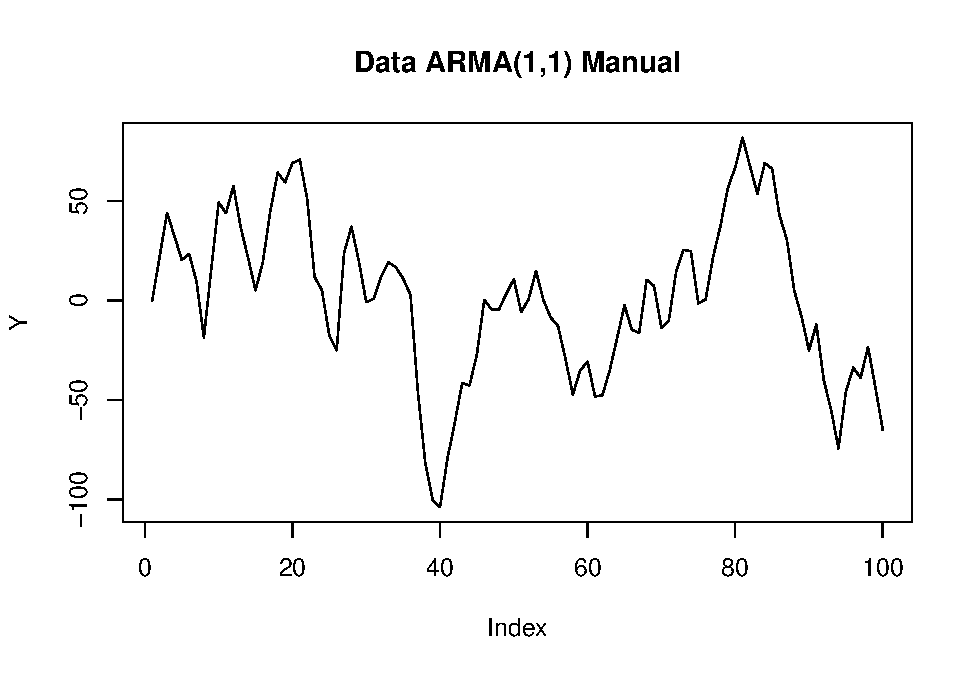
\includegraphics{_main_files/figure-latex/Membuat Data-1} 

}

\caption{Grafik Data Manual}(\#fig:Membuat Data)
\end{figure}
\begin{jp}{}{}
\begin{enumerate}
\item Berikan interpretasi anda mengenai grafik tersebut !  
\item Apakah data tersebar pada rataan data ?  
\item Apakah terdapat pola tren data ?
\end{enumerate}
\end{jp}

Berikutnya akan dicoba menghitung ACF secara manual

\begin{Shaded}
\begin{Highlighting}[]
\NormalTok{maxLag }\OtherTok{\textless{}{-}} \DecValTok{25}  
\NormalTok{acf\_manual }\OtherTok{\textless{}{-}} \FunctionTok{rep}\NormalTok{(}\DecValTok{1}\NormalTok{,maxLag)}
\ControlFlowTok{for}\NormalTok{(i }\ControlFlowTok{in} \DecValTok{1}\SpecialCharTok{:}\NormalTok{maxLag)\{}
\NormalTok{pembilang }\OtherTok{\textless{}{-}}\NormalTok{ (Y[}\DecValTok{1}\SpecialCharTok{:}\NormalTok{(n\_sim}\SpecialCharTok{{-}}\NormalTok{i}\SpecialCharTok{+}\DecValTok{1}\NormalTok{)]}\SpecialCharTok{{-}}\FunctionTok{mean}\NormalTok{(Y))}\SpecialCharTok{\%*\%}\NormalTok{(Y[i}\SpecialCharTok{:}\NormalTok{n\_sim]}\SpecialCharTok{{-}}\FunctionTok{mean}\NormalTok{(Y))}
\NormalTok{penyebut }\OtherTok{\textless{}{-}} \FunctionTok{sum}\NormalTok{((Y}\SpecialCharTok{{-}}\FunctionTok{mean}\NormalTok{(Y))}\SpecialCharTok{\^{}}\DecValTok{2}\NormalTok{)}
\NormalTok{acf\_manual[i]}\OtherTok{\textless{}{-}}\FunctionTok{sum}\NormalTok{(pembilang}\SpecialCharTok{/}\NormalTok{penyebut)}
\NormalTok{\}}
\NormalTok{acf\_r }\OtherTok{\textless{}{-}} \FunctionTok{as.vector}\NormalTok{(}\FunctionTok{acf}\NormalTok{(Y,}\AttributeTok{lag.max =} \DecValTok{24}\NormalTok{,}\AttributeTok{plot =}\NormalTok{ F)}\SpecialCharTok{$}\NormalTok{acf)}
\NormalTok{galat }\OtherTok{\textless{}{-}}\NormalTok{ acf\_manual }\SpecialCharTok{{-}}\NormalTok{ acf\_r}
\FunctionTok{sum}\NormalTok{(galat) }\CommentTok{\# Total Galat }
\end{Highlighting}
\end{Shaded}

\begin{verbatim}
## [1] -3.365364e-16
\end{verbatim}

Terakhir akan dicoba menghitung PACF secara manual. Perhatikan bahwa PACF dapat dituliskan dengan persamaan Yule Walker seperti berikut :
\begin{equation}
\rho_j = \phi_{k1} \rho_{j-1} + \phi_{k2} \rho_{j-2}+ \phi_{k3} \rho_{j-3} +\dots +\phi_{kk} \rho_{j-k}, \quad k \in \mathbb{N}
\end{equation}
Secara umum maka diperoleh
\begin{align*}
\phi_{k1} + \rho_1 \phi_{k2} + \rho_2 \phi_{k3} + \dots + \rho_{k-1} \phi_{kk}&= \rho_1 \\
\rho_1\phi_{k1} +  \phi_{k2} + \rho_1 \phi_{k3} + \dots + \rho_{k-2} \phi_{kk}&= \rho_2 \\
\rho_2\phi_{k1} +  \rho_1 \phi_{k2} + \phi_{k3} + \dots + \rho_{k-3} \phi_{kk}&= \rho_3 \\
\quad \quad \vdots \\
\rho_{k-1}\phi_{k1} +  \rho_{k-2}\phi_{k2} + \rho_{k-3} \phi_{k3} + \dots +  \phi_{kk}&= \rho_k \\
\end{align*}
Sehingga persamaan ini dapat ditulis menjadi persamaan matriks sebagai berikut :
\begin{equation}
\mathbf{A}\mathbf{x} = \mathbf{y}
\end{equation}
dengan masing - masing,
\begin{equation} 
\mathbf{A} = 
\begin{bmatrix}
1 &\rho_1 & \rho_2 & \dots & \rho_{k-1} \\
\rho_1 & 1 & \rho_1 & \dots & \rho_{k-2} \\
\rho_2 & \rho_1 & 1 & \dots & \rho_{k-3} \\ 
\vdots & \vdots & \ddots & \vdots & \vdots \\ 
\rho_{k-1}& \rho_{k-2} & \rho_{k-3} & \dots &1 
\end{bmatrix} 
\end{equation}
dan
\begin{equation}
\mathbf{x}=
\begin{bmatrix}
\phi_{k1}\\
\phi_{k2}\\
\phi_{k3}\\ 
\vdots \\
\phi_{kk} 
\end{bmatrix} \text{ dan } 
\mathbf{y} = 
\begin{bmatrix}
\rho_1 \\
\rho_2 \\ 
\rho_3 \\
\vdots \\
\rho_k
\end{bmatrix} 
\end{equation}
Sehingga untuk menghitung nilai dari \(\mathbf{x}\) dapat dilakukan dengan :
\begin{equation}
\mathbf{x} = \mathbf{A}^{-1}\mathbf{y}
\end{equation}
Ingat bahwa nilai korelasi parsial yang ingin dihitung adalah \(\phi_{kk}\) sehingga perhitungannya dapat dilakukan iterasi sebagai berikut :

\begin{Shaded}
\begin{Highlighting}[]
\FunctionTok{library}\NormalTok{(matrixcalc) }\CommentTok{\# Untuk mencari invers matriks}
\end{Highlighting}
\end{Shaded}

\begin{verbatim}
## Warning: package 'matrixcalc' was built under R version 4.2.1
\end{verbatim}

\begin{Shaded}
\begin{Highlighting}[]
\NormalTok{maxLag }\OtherTok{\textless{}{-}} \DecValTok{24} \CommentTok{\# Ukuran vektor dan matriks}
\NormalTok{pacf\_manual }\OtherTok{\textless{}{-}} \FunctionTok{rep}\NormalTok{(}\DecValTok{0}\NormalTok{,maxLag)}
\ControlFlowTok{for}\NormalTok{ (k }\ControlFlowTok{in} \DecValTok{1}\SpecialCharTok{:}\NormalTok{maxLag)\{}
\ControlFlowTok{if}\NormalTok{ (k }\SpecialCharTok{==}\DecValTok{1}\NormalTok{)\{}
\NormalTok{  pacf\_manual[k] }\OtherTok{\textless{}{-}}\NormalTok{ acf\_r[}\DecValTok{2}\NormalTok{] }\CommentTok{\# Hati {-} hati }
\NormalTok{\}                   }\CommentTok{\#jika mau mengubah maxLag}
\ControlFlowTok{else}\NormalTok{\{}
\NormalTok{rho }\OtherTok{\textless{}{-}}\NormalTok{ acf\_r[}\DecValTok{1}\SpecialCharTok{:}\NormalTok{(k}\SpecialCharTok{+}\DecValTok{1}\NormalTok{)] }\CommentTok{\# Vektor y}
\NormalTok{phi }\OtherTok{\textless{}{-}} \FunctionTok{matrix}\NormalTok{(}\DecValTok{1}\NormalTok{, }\AttributeTok{nrow=}\NormalTok{k,}\AttributeTok{ncol=}\NormalTok{k) }\CommentTok{\# Matriks A}
\ControlFlowTok{for}\NormalTok{ (i }\ControlFlowTok{in} \DecValTok{1}\SpecialCharTok{:}\NormalTok{(k))\{}
  \ControlFlowTok{for}\NormalTok{ (j }\ControlFlowTok{in} \DecValTok{1}\SpecialCharTok{:}\NormalTok{(k))\{}
\NormalTok{    phi[i,j] }\OtherTok{\textless{}{-}}\NormalTok{ rho[}\FunctionTok{abs}\NormalTok{(i}\SpecialCharTok{{-}}\NormalTok{j)}\SpecialCharTok{+}\DecValTok{1}\NormalTok{] }\CommentTok{\# Membuat matriks simetri}
\NormalTok{  \}}
\NormalTok{\}}\CommentTok{\# vektor x}
\NormalTok{pacf\_manual[k] }\OtherTok{\textless{}{-}} \FunctionTok{as.vector}\NormalTok{(}\FunctionTok{matrix.inverse}\NormalTok{(phi)}\SpecialCharTok{\%*\%}\NormalTok{rho[}\DecValTok{2}\SpecialCharTok{:}\NormalTok{(k}\SpecialCharTok{+}\DecValTok{1}\NormalTok{)])[k] }
\NormalTok{\}}
\NormalTok{\}}
\NormalTok{pacf\_r }\OtherTok{\textless{}{-}} \FunctionTok{as.vector}\NormalTok{(}\FunctionTok{acf}\NormalTok{(Y,}
                      \AttributeTok{lag.max =}\NormalTok{ maxLag, }
                      \AttributeTok{type =} \StringTok{\textquotesingle{}partial\textquotesingle{}}\NormalTok{,}
                      \AttributeTok{plot =}\NormalTok{ F)}\SpecialCharTok{$}\NormalTok{acf)}
\NormalTok{galat }\OtherTok{\textless{}{-}}\NormalTok{ pacf\_manual }\SpecialCharTok{{-}}\NormalTok{ pacf\_r}
\FunctionTok{sum}\NormalTok{(galat) }\CommentTok{\# Total Galat }
\end{Highlighting}
\end{Shaded}

\begin{verbatim}
## [1] -1.39385e-15
\end{verbatim}

  \bibliography{book.bib,packages.bib}

\end{document}
